\documentclass[aspectratio=10]{beamer} %For normal presentation (comment otherwise)
%\documentclass[aspectratio=169]{beamer} %for widescreen prestentation
\usetheme{Marburg}
\usefonttheme{serif}
\usecolortheme{default}%albatross, crane, beetle, dove, fly, seagull, wolverine e beaver.
%%%%%%%%%%%%%%%%%%%%%%%%%%%%%%%%%%%%%%%%%%%%%%%%%%%%%%%%%%%%%%%%%%%%%%%%%%%%%%%%%%%%%%%%%%%%%%%
%%%%%%%%%%%%%%%%%%%%%%%%%%%%%%%%%%%%%%EXTRA PACTAGES%%%%%%%%%%%%%%%%%%%%%%%%%%%%%%%%%%%%%%%%%%%
\usepackage[utf8]{inputenc}
\usepackage[T1]{fontenc}
\usepackage[portuguese, english]{babel}
\usepackage[round]{natbib}
\usepackage{hyperref} 
\usepackage{tcolorbox}
\usepackage{graphicx} % Required for including images
\usepackage{graphics}
\graphicspath{{Imagens/}} % Location of the graphics files
\usepackage{booktabs} % Top and bottom rules for table
\usepackage[font=small,labelfont=bf]{caption}%specifies captions on tables and figures
\usepackage{amsfonts, amsmath, amsthm, amssymb} % For math fonts, symbols and environments
\usepackage{wrapfig} % Allows wrapping text around tables and figures
\usepackage{makeidx}
\usepackage{lipsum} % Required to insert dummy text. To be removed otherwise
\usepackage{epstopdf}%adiciona imagens em formato eps no pdf.
\usepackage{subfigure}%cria ambientes de multifiguras
\usepackage{float}%coloca as figuras exatamente aonde você quer
\usepackage{times}
\usepackage{tikz}%pacote para fazer fluxogramas
\usepackage{verbatim}%
\usepackage{smartdiagram}
%%%%%%%%%%%%%%%%%%%%%%%%%%%%%%%%%%%%%%%%%%%%%%%%%%%%%%%%%%%%%%%%%%%%%%%%%%%%%%%%%%%%%%%%%%%%%
%%%%%%%%%%%%%%%%%%%%%%%%%%%%%%%%%%%%%PREAMBLE%%%%%%%%%%%%%%%%%%%%%%%%%%%%%%%%%%%%%%%%%%%%%%%%
\author[Carreira,V.R.]{Authors: Victor Ribeiro Carreira$^{1}$, Cosme Ferreira Ponte Neto$^{1}$, Rodrigo Bijani Santos$^{1}$}
\title{A Comparison of Machine Learning Processes for Classification of Rock Units Using Well Log Data}
%\subtitle{}
\institute{Observatório Nacional$^{1}$}
\date{June 2018}
\subject{EAGE  ANNUAL 80TH CONFERENCE + EXHIBITION. COPENHAGEN, DENMARK. 2018}
%\setbeamertemplate{footline}[frame number]
%\setbeamercovered{transparent}
%\setbeamertemplate{navigation symbols}{}
% Tela cheia
\hypersetup{pdfpagemode=FullScreen}
\usepackage{ragged2e}
\justifying
\addtobeamertemplate{headline}{} 
{\begin{tikzpicture}[remember picture, overlay]
	\node [anchor=south west, inner sep=0.4cm]  at (current page.south west)
	{
\includegraphics[height=0.4cm]{Imagens/eage18.eps}};
	\end{tikzpicture}}
%%%%%%%%%%%%%%%%%%%%%%%%%%%%%%%%%%%%%%%%%%%%%%%%%%%%%%%%%%%%%%%%%%%%%%%%%%%%%%%%%%%%%%%%%%%%%%%%%%%%%%%%%%%%%%%%%%%%%%%%%%%%%%%%%%%%%%PRESENTATION%%%%%%%%%%%%%%%%%%%%%%%%%%%%%%%%%%%%%%%%%%%%%%%%%%%%%%%%%%%%%%%%%%%%%%%%%%%%%%%%%%%%%%%%%%%%%%%%%%%%%%%%%%%%%%%%%%%%%%%%%%%%%%%%%%%%%%%%%%%
\begin{document}

	\bgroup
	\makeatletter
	\setbeamertemplate{footline}
	\makeatother

%\maketitle
\egroup 
\addtobeamertemplate{navigation symbols}{}{\hskip6pt\raisebox{2pt}{\color{blue}\insertframenumber}}
\setcounter{framenumber}{-1}
\AtBeginSection[]


\begin{frame}
 \flushbottom
 \setlength{\parskip}{-1ex plus 1ex }
 \setlength{\parindent}{-15pt}
 
\includegraphics[width=13cm,height=10cm]{Imagens/front.pdf}
\end{frame}


\section{Introduction}

\subsection{Motivation}


{%
	\usebackgroundtemplate{
		\centering
		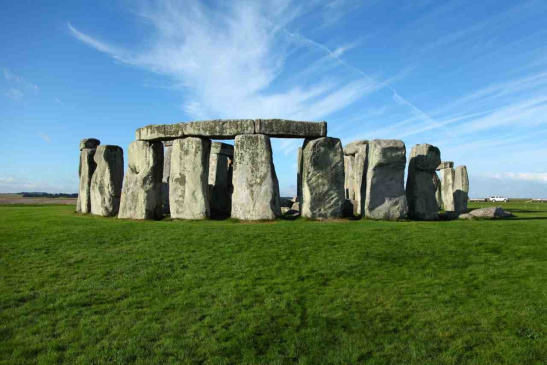
\includegraphics[width=\paperwidth,height=\paperheight]{Imagens/stonerange.jpg}
	}
	
	% Frame 3: plano de fundo
	\begin{frame}
	\frametitle{\textcolor{yellow}{Changing seasons}}
	%\flushbottom\color{yellow}{\normalsize Changing seasons}
	
\end{frame}
}

{%
\usebackgroundtemplate{
	\centering
	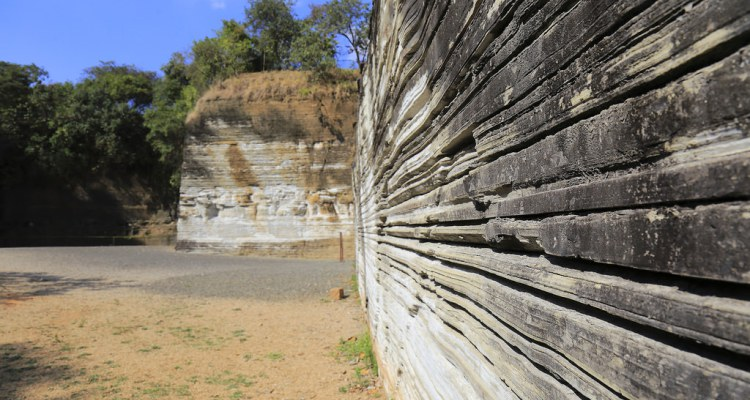
\includegraphics[width=\paperwidth,height=\paperheight]{Imagens/varvite.jpg}
}

% Frame 3: plano de fundo
\begin{frame}
\frametitle{\textcolor{yellow}{Varvite (Itu - São Paulo)}}
%\flushbottom\color{yellow}{\normalsize Changing seasons}

\end{frame}
}


\begin{frame}
\frametitle{Introduction}
\begin{columns}
	\column{0.55\textwidth}
		\footnotesize
		\justifying
		\begin{itemize}
		\item[Machine learning:] computer program with capability of automatic improvement trought experience.
		\pause
		\item[Machine learning groups:]
		   \begin{enumerate}
			 {\tiny 
			 	\item  Artifitial Neural Networks \citep{Minsky1969,Michie1994,MacKay2005};
			    \item Decision trees \citep{Mitchell1997,Simard2000,Roberts2002};
			    \item Statistical Classifiers \citep{Michel2016};
			    \item Self-Organizing Maps \citep{Kohonen1989,Haykin1999};
			}
		   \end{enumerate}
		\pause
		\item[Classifiers:] uses the concept of distance in the space of attributes;
		\pause
		\item[Euclidean classifier:] calculates a centroid in the space of attributes.
		\pause
		\item[Mahalanobis classifier:] takes into consideration the shape of attributes space.
		\pause
		\item[Self-Organizing Map:] inspired by neural cortex and based oriented graph that works as an interconnected network. 
	\end{itemize}
\end{columns}
\end{frame}

\subsection{Objective}
\begin{frame}
\frametitle{Objective of this work}
\begin{columns}\footnotesize 
	\justifying
	\column{0.55\textwidth}
	\begin{itemize}
		\item[Geosphysical problem:] Identify rocks from well log data by means of machine learning and statistical classifiers;
		\pause
		\item[Way to solve it:] use self-organizing map (SOM) and two statistical classifers;
		\pause
		\item[Strategy:] Compare the results for the three explored methods, Kohonen (SOM), euclidean and mahalanobean classifiers for a synthetic scenarium.
	\end{itemize}
\end{columns}
\end{frame}


\section{Methodology}

\subsection{Synthetic Sedimentary Basin}

\begin{frame}
	\frametitle{Synthetic Sedimentary Basin}
	\begin{figure}[H]
		\centering
		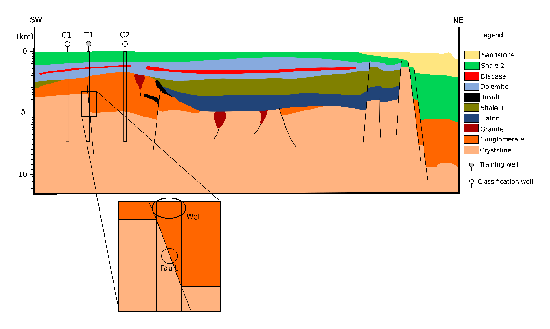
\includegraphics[scale=0.34]{Imagens/Basin.eps}
		\caption{\footnotesize Synthetic Sedimentary Basin by \cite{Sal2008}  T1, C1 and C2 are training and classifing wells respectively.}
		\label{Model}
	\end{figure}
\end{frame}

\begin{frame}
\frametitle{Synthetic Sedimentary Basin}
\begin{table}[H]\tiny
	\caption{Physical properties and rock types.}
\begin{tabular}{@{}ccccccccccc@{}}
	\toprule
	Rock & Density ($g/cm^{3}$) & Gamma ray ($Ci/g$) & Resistivity ($\Omega.m$)& Velocity ($Km/s$) &\\ \midrule
	Conglomerate &     $2.30$ 		  &       $100.0$       &           $6000$           &			$2$   		   	&\\
	Shale	 &       $2.55$           &       $100.0$       &           $1000$           &     		$3$		 &\\
	Dolomite     &       $2.72$           &       $8.30$        &           $3.5 \times 10^{3}$           &  	$6$    			 &\\
	Diabase    &       $2.91$           &       $30.0$        &           $15 \times 10^{7}$           &      $5.5$				 &\\
	Crystalline  &       $2.80$           &       $0.7$         &           $1.3 \times 10^{6}$           & 		$5$		     &\\ \bottomrule
\end{tabular}

\label{Tab1}
\end{table}
\begin{columns}
	\column{0.55\textwidth}
	\footnotesize
	\justifying
\begin{itemize}\footnotesize
	\item[Sample rate:] $0.01$ observation/meter 
	\item[Contamination error:] $5$\% Radom Gaussian noise.
\end{itemize}
\end{columns}
\end{frame}

\begin{frame}
	\frametitle{Methodology}
	\smartdiagram[priority descriptive diagram]{
		Generates the hypothesis model,
		Uses T1 well data to train the Kohonen (SOM) and make the statistical of classifiers,
		Uses C1 and C2 to make predictions using SOM and the classifiers,
		Compare the results					}
\end{frame}

\subsection{Training and Similarities}

\begin{frame}
	\frametitle{Training and Similarities}
	\begin{figure}[H]
		\centering
		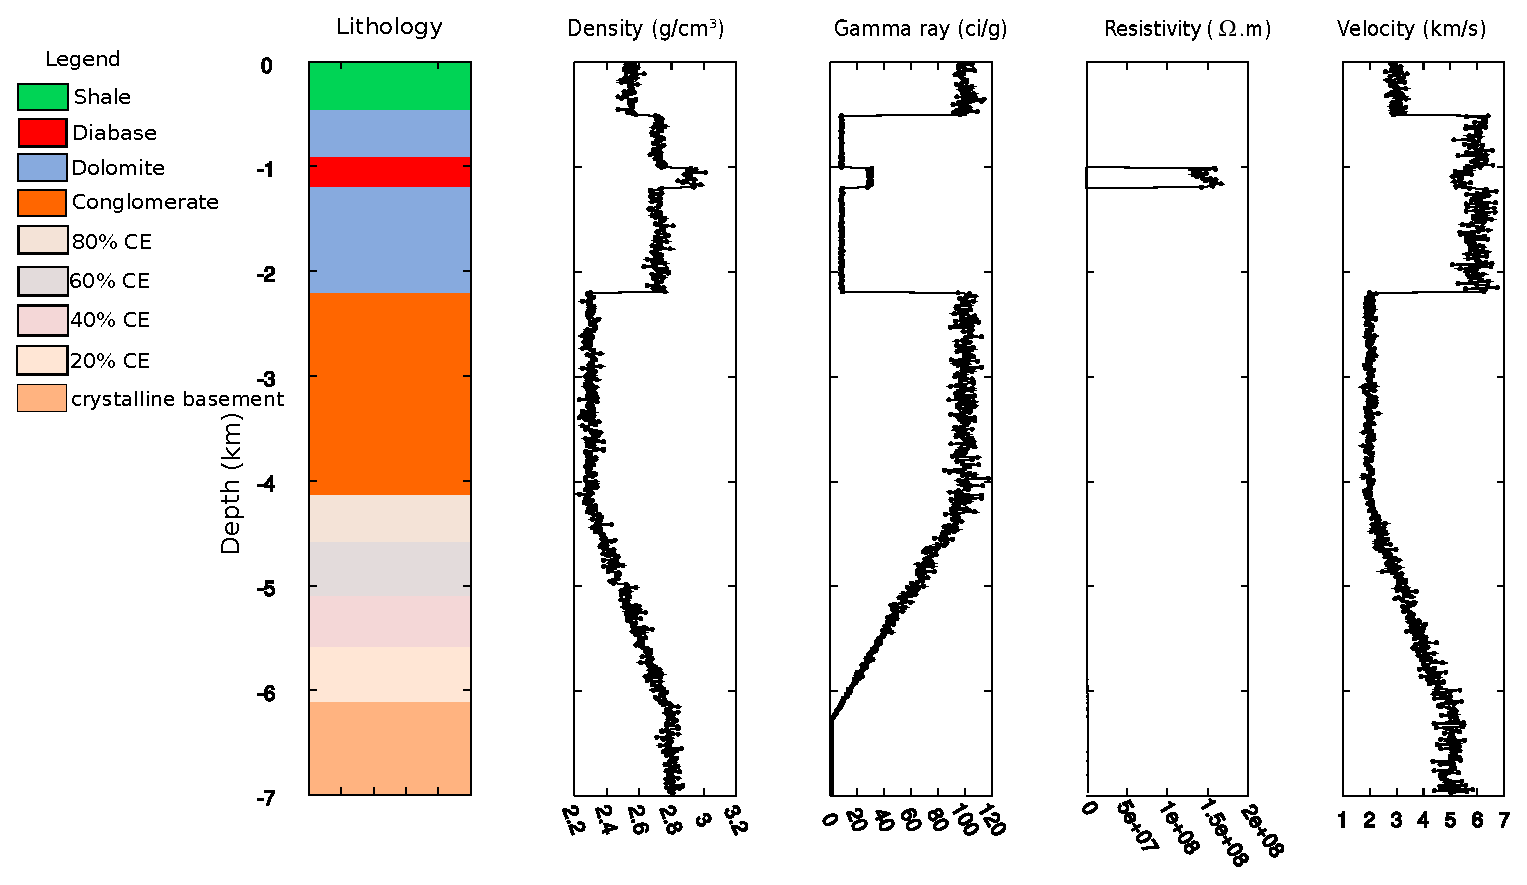
\includegraphics[scale=0.34]{Imagens/Pocot1.eps}
		\caption{Synthetic training well T$1$.}
		\label{T1}
	\end{figure}
\pause
\begin{itemize}\footnotesize
	\item Four divisions describes the normal fault by decreasing the amount of conglomerate in comparison to crystalline basement.
\end{itemize}

\end{frame}

\begin{frame}
\frametitle{Training and Similarities}
\begin{figure}[H]
	\centering
	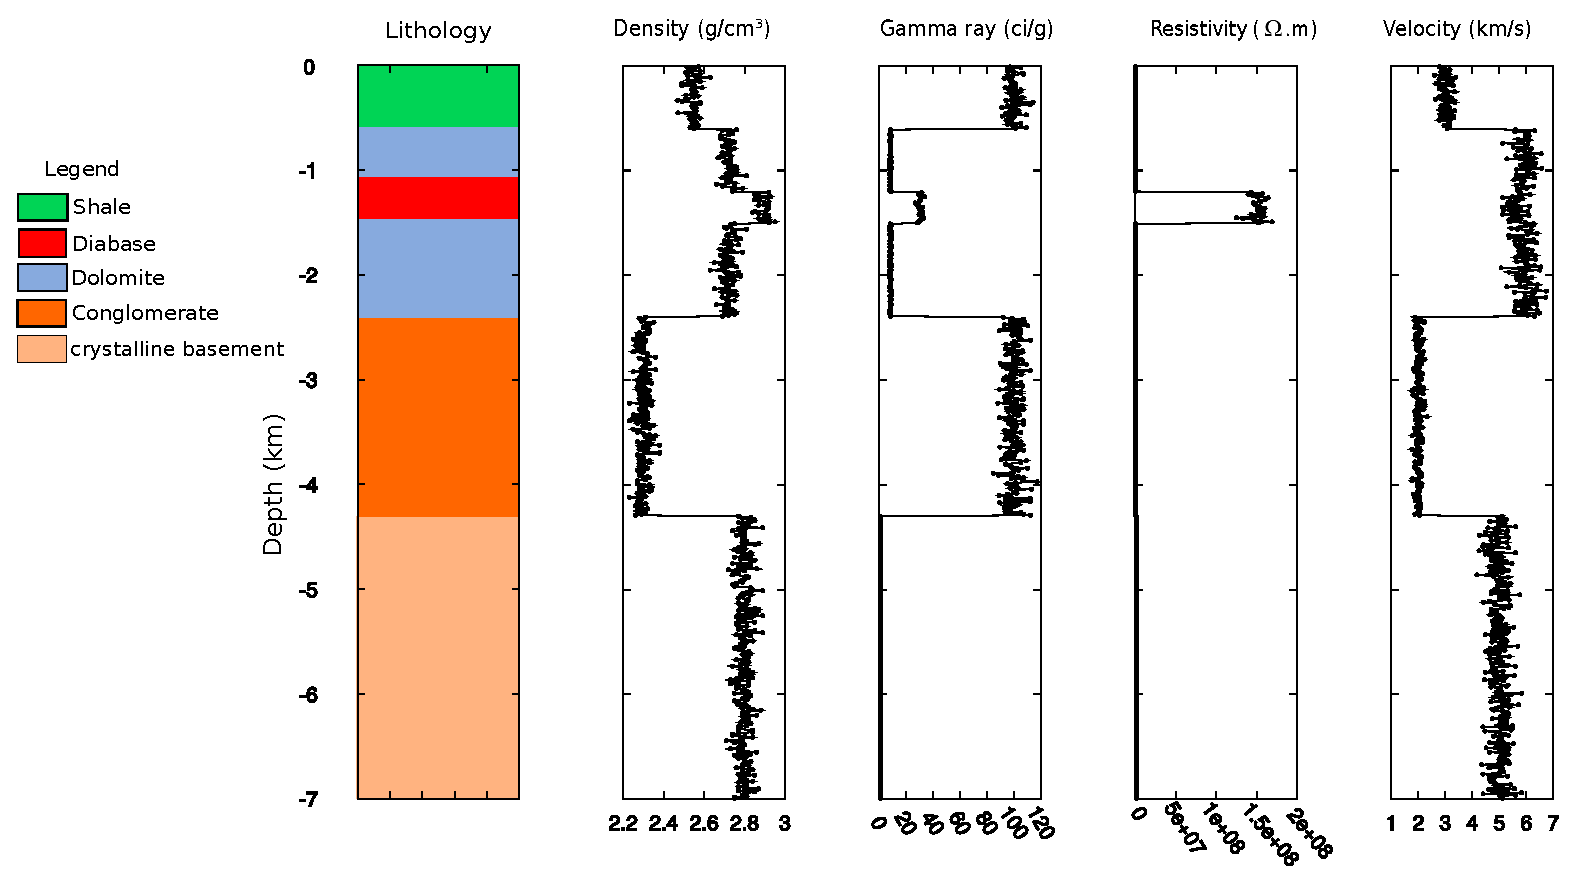
\includegraphics[scale=0.39]{Imagens/Pococ1.eps}
	\caption{Classification well C$1$}
	\label{C1}
\end{figure}
\end{frame}

\begin{frame}
\frametitle{Training and Similarities}
\begin{figure}[H]
	\centering
	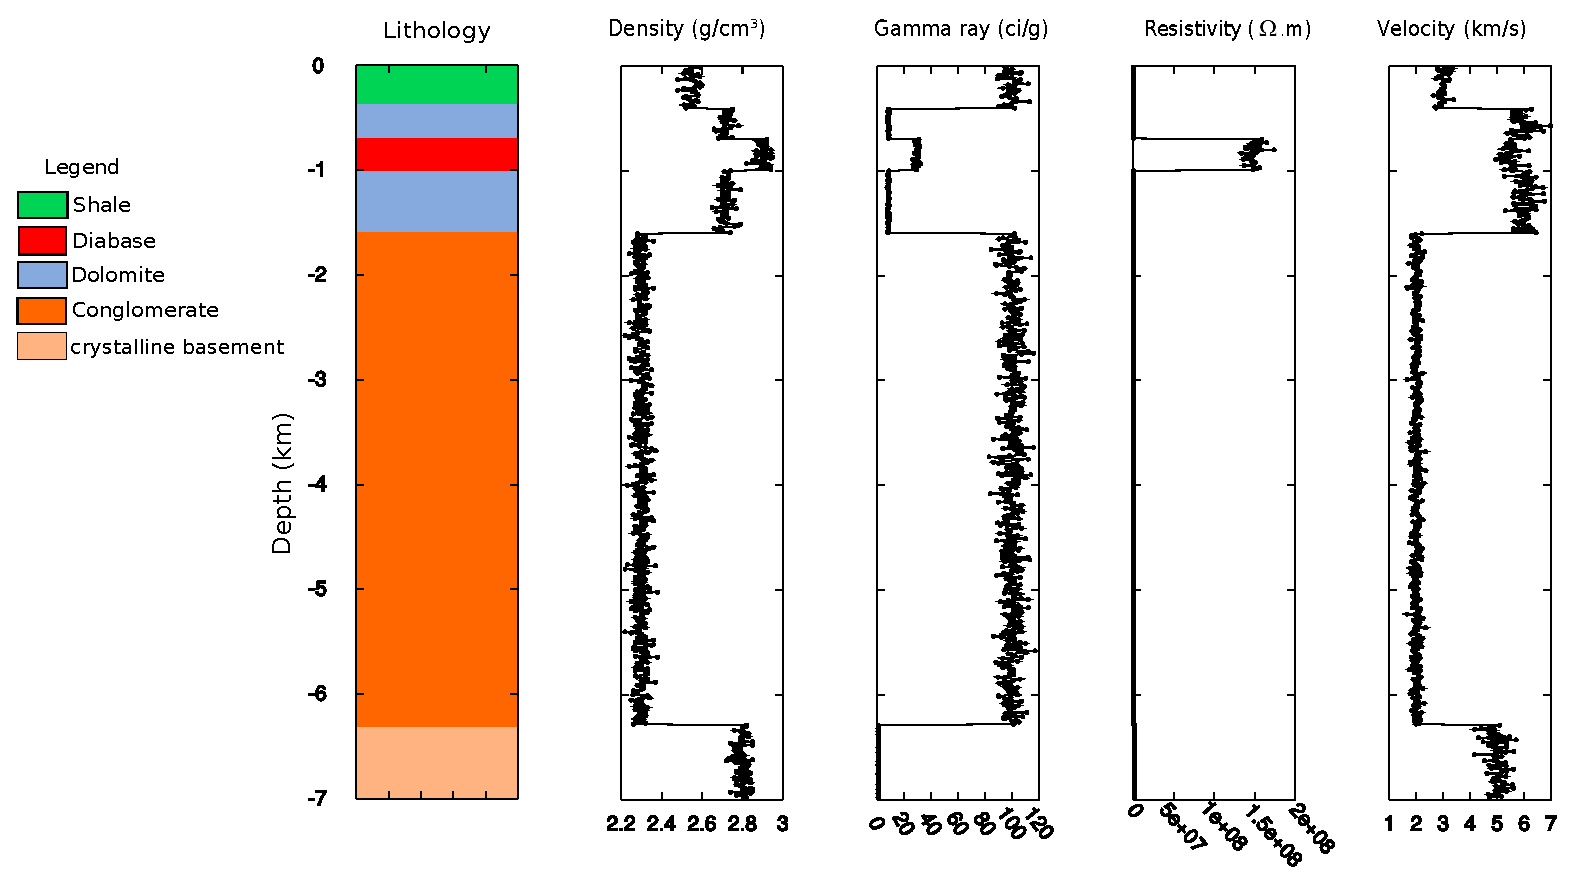
\includegraphics[scale=0.39]{Imagens/Pococ2.eps}
	\caption{Classification well C$2$}
	\label{C2}
\end{figure}
\end{frame}



\subsubsection{Euclidean Classifier}

\begin{frame}
	\frametitle{Euclidean Classifier}
		\begin{tcolorbox}[colback=gray!5,colframe=blue!40!black,title=Definition]
	\begin{equation}
	Ed_{i} =  \Arrowvert \textbf{X}-\bar{\textbf{X}}_{i}  \Arrowvert_{2} \nonumber
	\label{eq4}
	\end{equation}  
\end{tcolorbox}
	 \pause
	\begin{itemize}
		\centering
		\item[$\textbf{X}$], input vector (attribute data)
		\pause
		\item[$\bar{\textbf{X}}_{i}$], mean vector
	\end{itemize}
	
\end{frame}
  

\begin{frame}
  \frametitle{Euclidean Classifier}
    \begin{figure}[H]
    	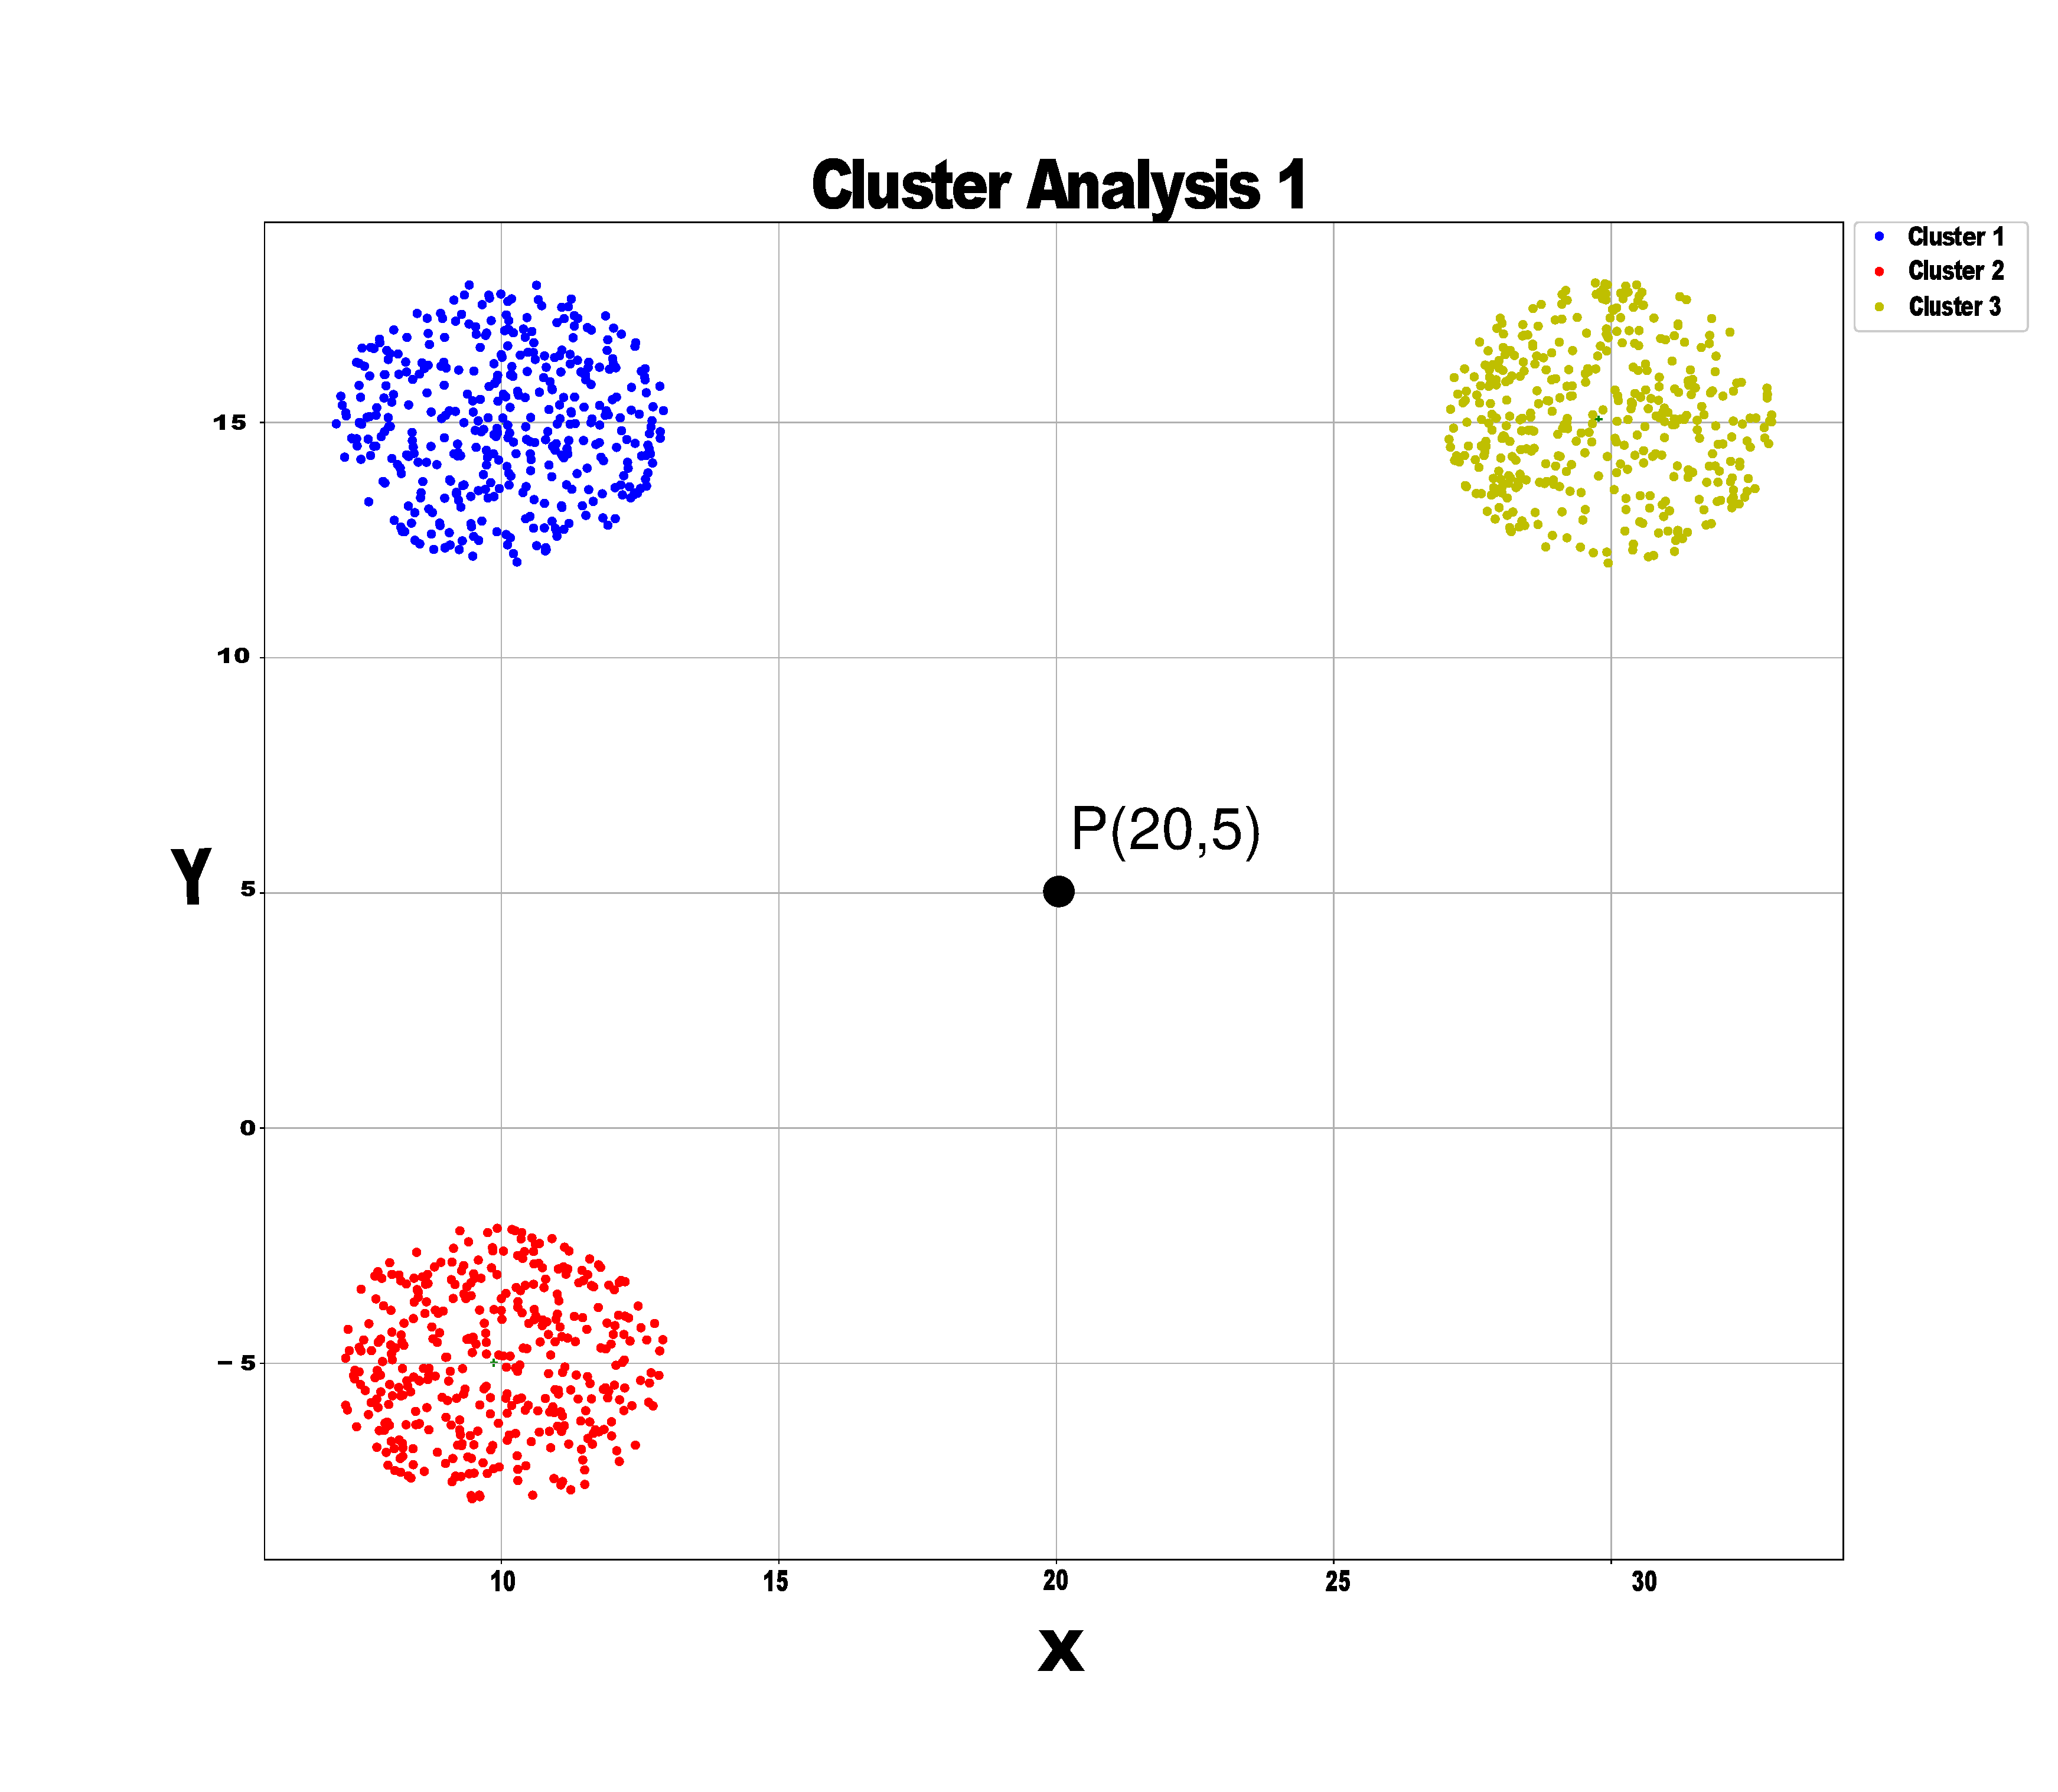
\includegraphics[scale=0.1]{Imagens/clusteranalise1.eps}
    \end{figure}
    
    \begin{columns}
    	\column{1\textwidth}
    	\footnotesize
    	\justifying
    \begin{itemize}
    	\footnotesize
    	\item All centroid are equidistant
    	\pause
    	\item P$(20,5)$ could be a member of all groups from a euclidean point of view 
    \end{itemize}
    \end{columns}
  
\end{frame}

\begin{frame}
\frametitle{Euclidean Classifier}
\begin{figure}[H]
	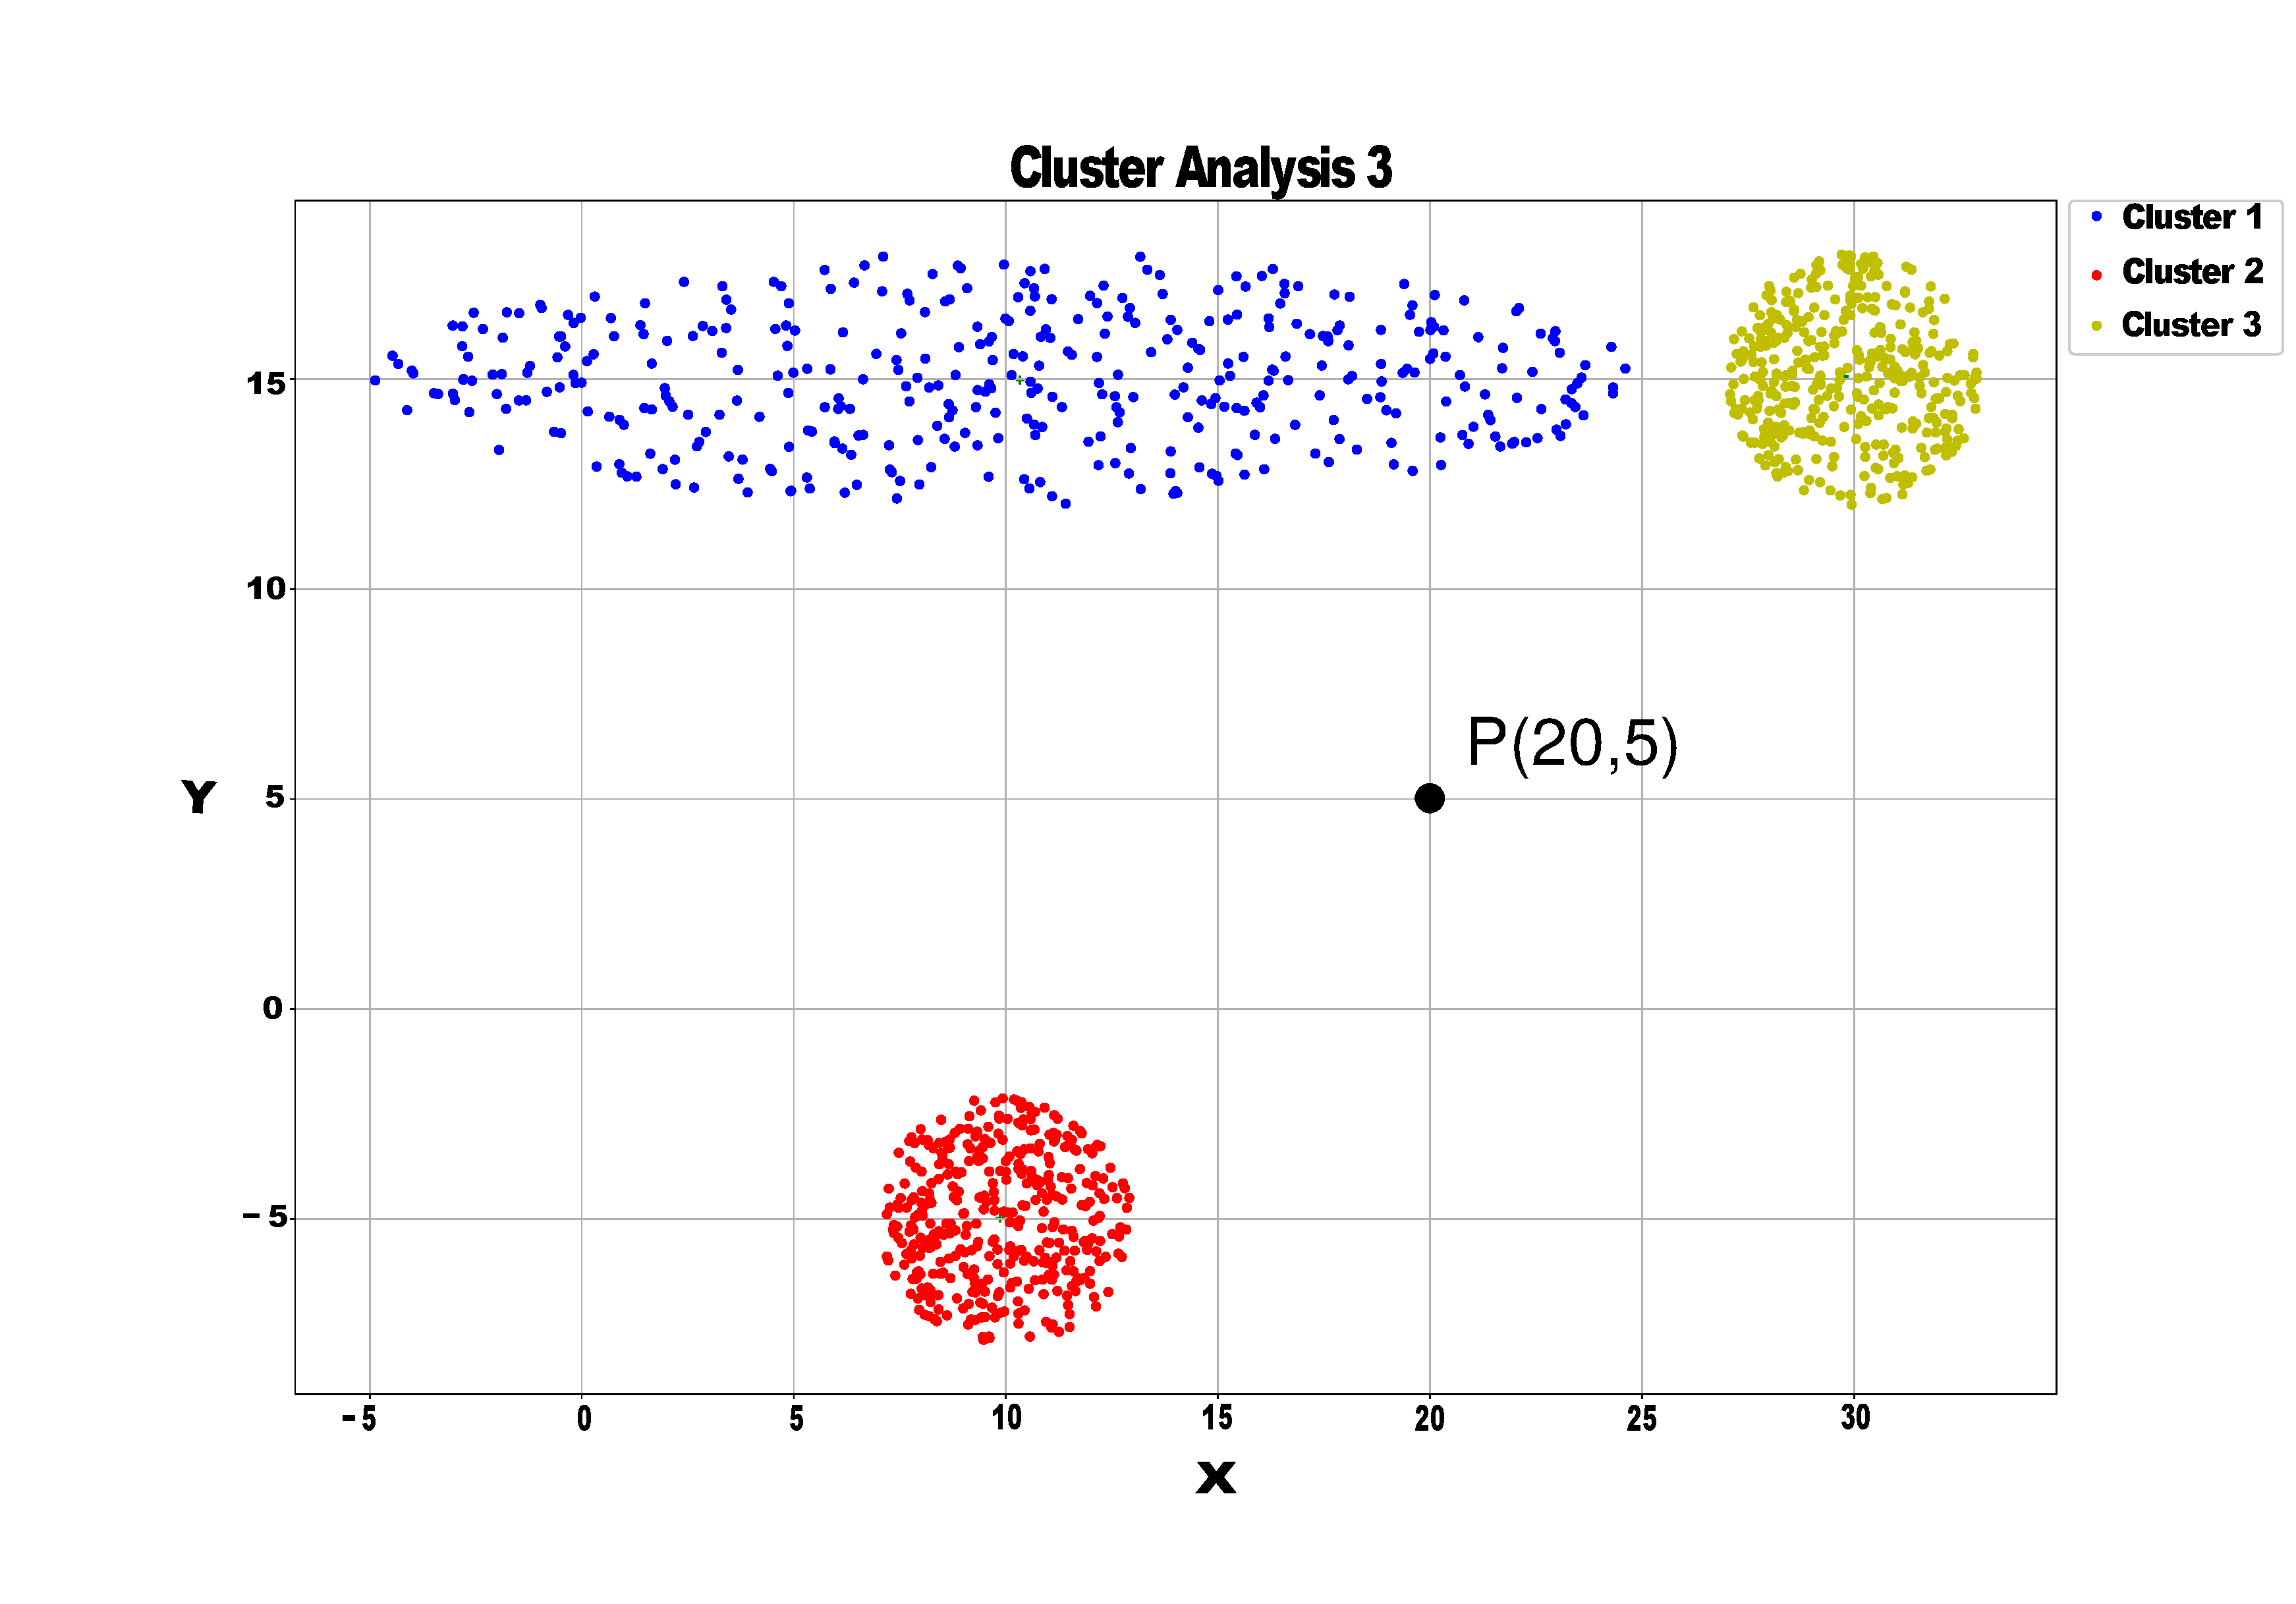
\includegraphics[scale=0.12]{Imagens/clusteranalise3.eps}
\end{figure}

    \begin{columns}
    	\column{1\textwidth}
    	\footnotesize
    	\justifying
\begin{itemize}
	\item Blue cluster still have the same centroid
	\pause 
	\item Problematic to define which cluster point P$(20,5)$ should be member of 
	\pause
	\item How could we handle this problem?
\end{itemize}
\end{columns}
\end{frame}

\subsubsection{Mahalanobis Classifier}

\begin{frame}
	\frametitle{Mahalanobis Classifier}
	\begin{tcolorbox}[colback=gray!5,colframe=blue!40!black,title=Definition]
	  \begin{equation}
			Md_{i}=\Arrowvert(\textbf{X}-\bar{\textbf{X}}_{i})^{T}\textbf{C}_{i}^{-1}(\textbf{X}-\bar{\textbf{X}}_{i})\Arrowvert_{2}\nonumber
			\label{eq5}
		\end{equation}
	\end{tcolorbox}
	 \pause
	\begin{itemize}
		\centering
    	\item[$\textbf{X}$], input vector 
		\pause
		\item[$\bar{\textbf{X}}_{i}$], mean vector
		\pause
		\item[$\textbf{C}_{i}$], covariance matrix
	\end{itemize}
\end{frame}


%\begin{frame}
%\frametitle{Mahalanobis Classifier}
%
%\begin{equation}
%\textbf{C}_{i}=\frac{1}{n_{i}-1}\sum_{X \in \omega_{i}}(\textbf{X}-\bar{\textbf{X}}_{i})(\textbf{X}-\bar{\textbf{X}}_{i})^{T}
%\label{eq6}
%\end{equation}
%\pause
%\begin{itemize}
%	\centering
%	\item[$n_{i}$], number of elements  
%	\pause
%	\item[$\omega_{i}$], space of attributes
%\end{itemize}
%\end{frame}

\begin{frame}
	\frametitle{Euclidean Classifier}
	\begin{figure}[H]
		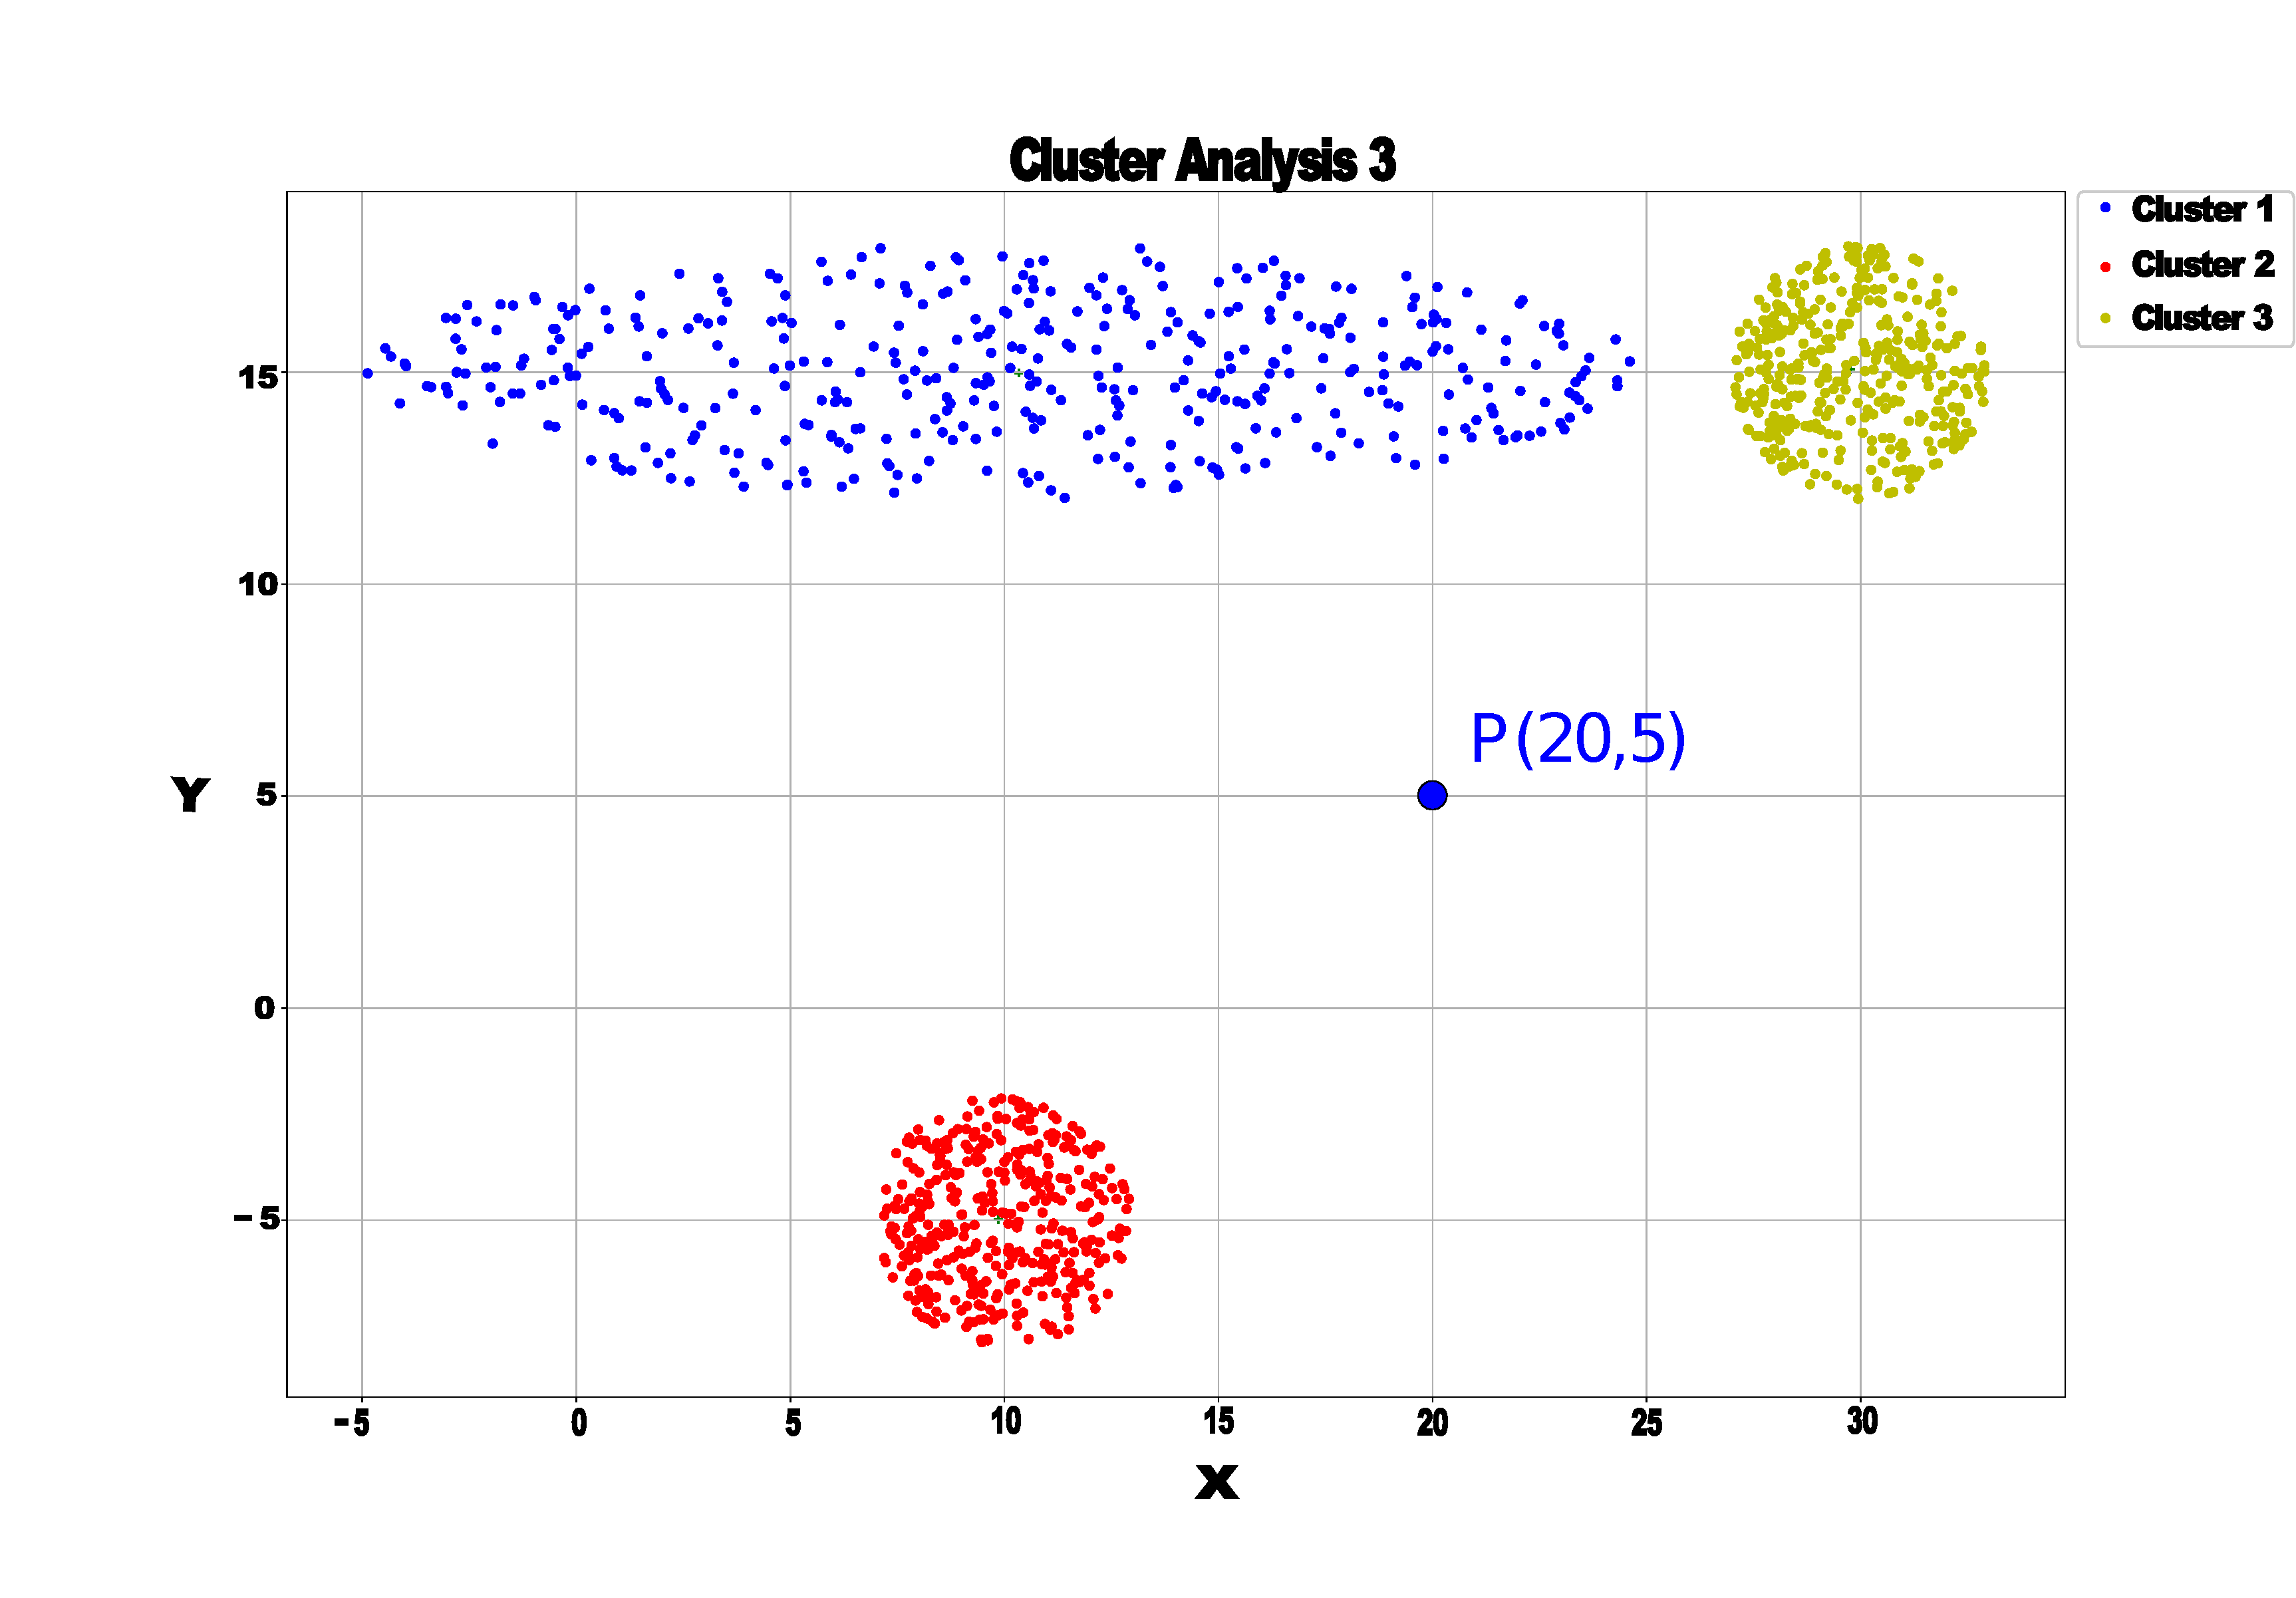
\includegraphics[scale=0.14]{Imagens/clusteranalise3blue.pdf}
	\end{figure}
	
	\begin{columns}
		\column{1\textwidth}
		\footnotesize
		\justifying
		\begin{itemize}
			\item Now, P$(20,5)$ belongs to  \textcolor{blue}{cluster $1$}.
		\end{itemize}
	\end{columns}
\end{frame}

\begin{frame}
	\begin{huge}
		\centering
		Back to the problem ...
	\end{huge}
\end{frame}

\subsubsection{Clusters and Space of Attributes}

\begin{frame}
	\frametitle{Cluster analysis for the syntetic example: T1 well}
	      \begin{columns}
	       	\column{0.5\textwidth}
	       	\footnotesize
	       	\justifying
	        \begin{figure}
	       %\centering
	       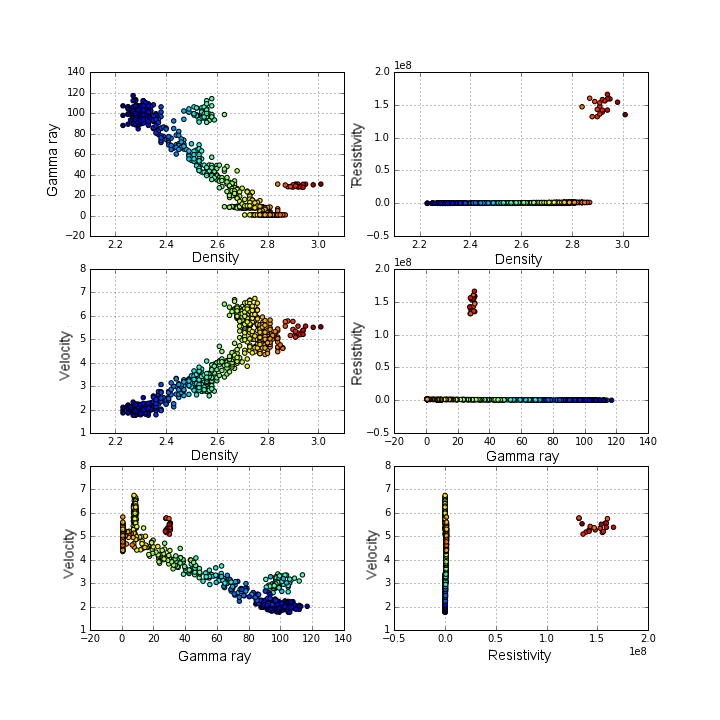
\includegraphics[scale=0.268]{Imagens/cluterpocoT1.png}
	       \end{figure}
	       
	       \column{0.3\textwidth}
	       \begin{itemize}
	       	\footnotesize
	       	\item Scatter plot in pairs ($6$ plots);
	       	\pause
	       	\item colors represents the variation rate of physical properties;
	       	\pause
	       	\item some elongated clusters;
	       	\pause
	       	\item some mixed clusters.
	       \end{itemize}
	       
         \end{columns}
\end{frame}


\begin{frame}
\frametitle{Clusters analysis for the example: C1 well}

     \begin{columns}
    	\column{0.5\textwidth}
     	\footnotesize
     	\justifying
     	\begin{figure}
    		%\centering
      		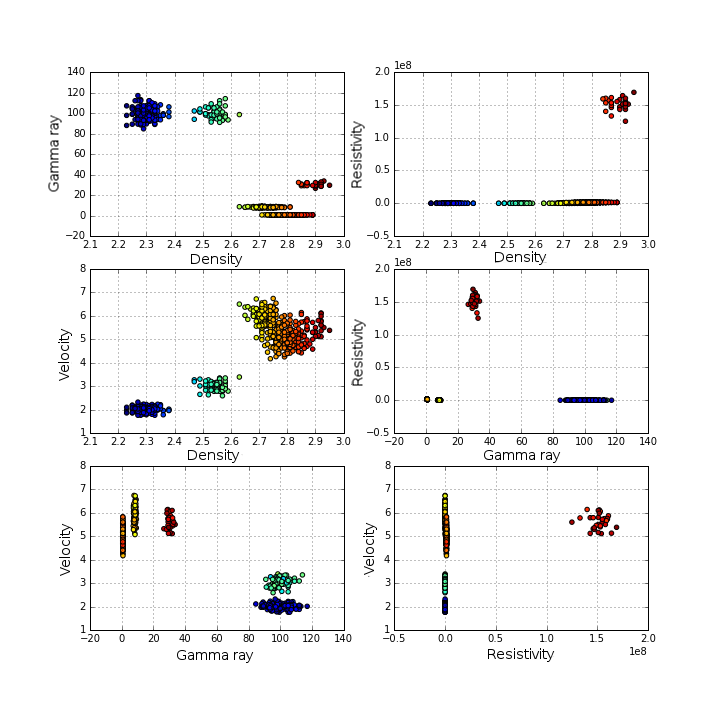
\includegraphics[scale=0.268]{Imagens/cluterpocoC1.png}
      	\end{figure}
      	
      	\column{0.3\textwidth}
      	\begin{itemize}
      		\footnotesize
      		\item Defined clusters;
      		\pause
      		\item Different from training well
    	\end{itemize}
      	
      \end{columns}
\end{frame}

\begin{frame}
\frametitle{Clusters analysis for the example: C2 well}

     \begin{columns}
     	\column{0.5\textwidth}
     	\footnotesize
     	\justifying
     	\begin{figure}
     		%\centering
     		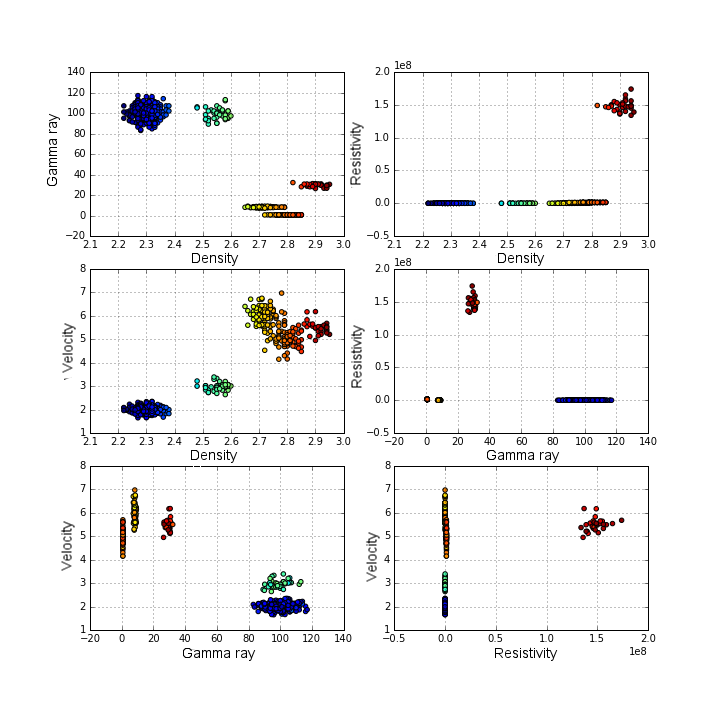
\includegraphics[scale=0.268]{Imagens/cluterpocoC2.png}
     	\end{figure}
     	
     	\column{0.3\textwidth}
     	\begin{itemize}
     		\footnotesize
     		\item Similar to C1 well
     	\end{itemize}
     	
     \end{columns}
\end{frame}

\subsubsection{Kohonen - SOM}


\begin{frame}
  \frametitle{Kohonen - SOM}
  \framesubtitle{Organization}
  	 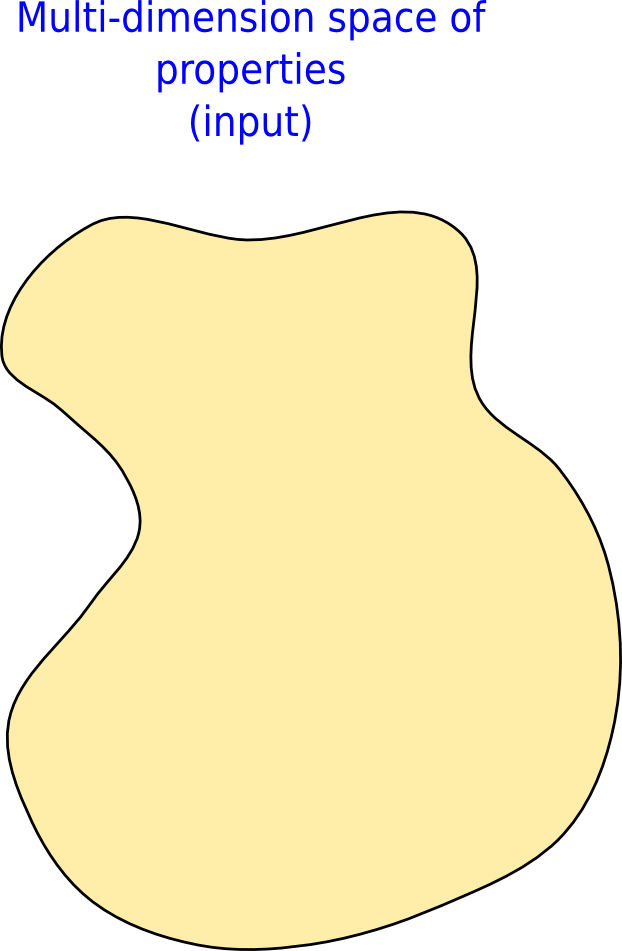
\includegraphics[scale=0.5]{Imagens/Introkoho1.png} 
\end{frame}


\begin{frame}
  \frametitle{Kohonen - SOM}
  \framesubtitle{Organization}
 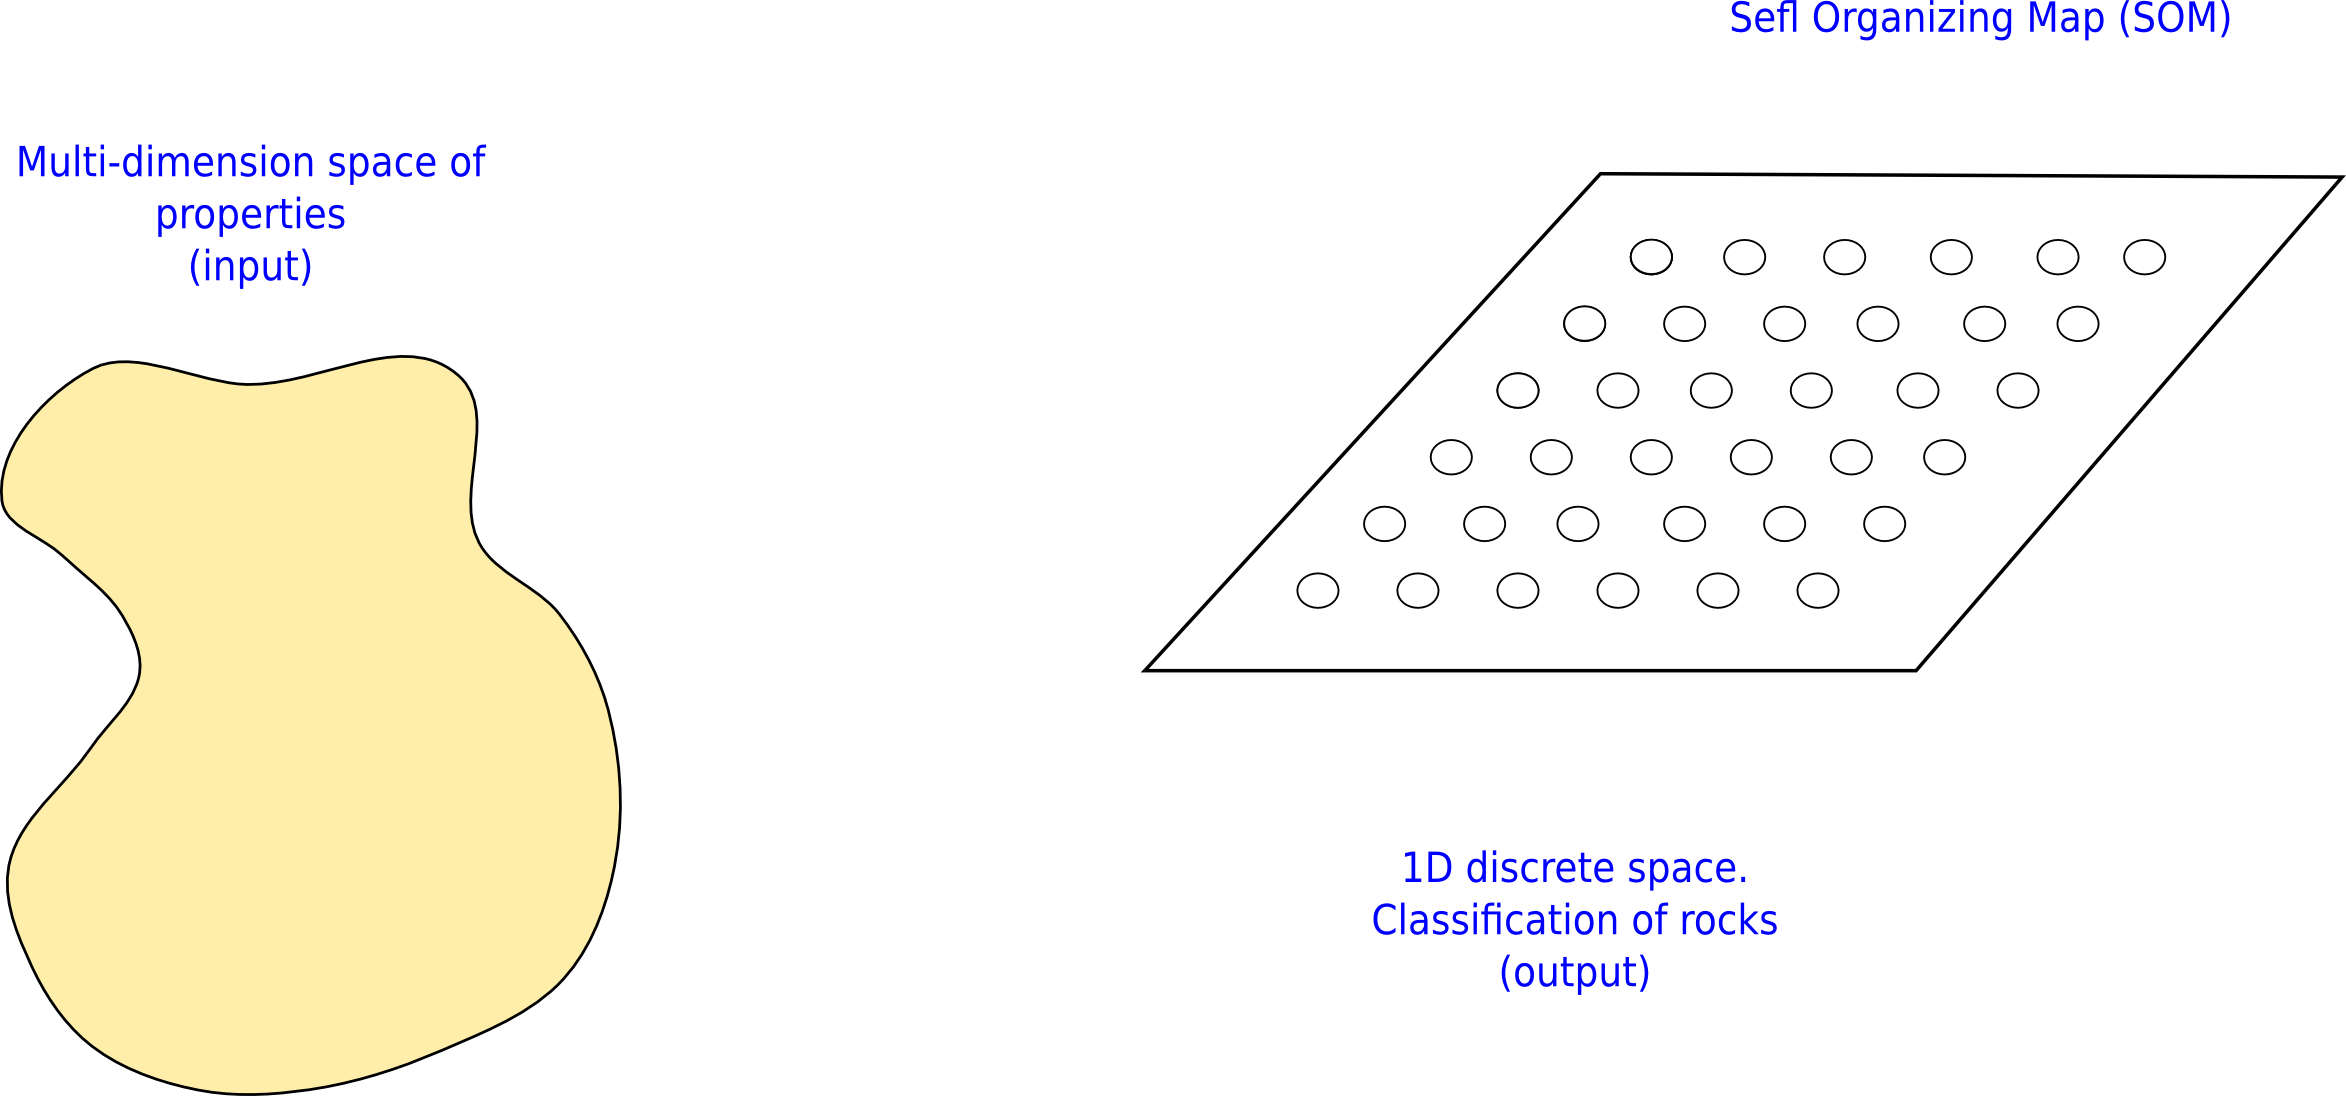
\includegraphics[scale=0.5]{Imagens/Introkoho2.png} 
\end{frame}


\begin{frame}
 \frametitle{Kohonen - SOM}
 \framesubtitle{Synaptic adaptation (Training process)}
 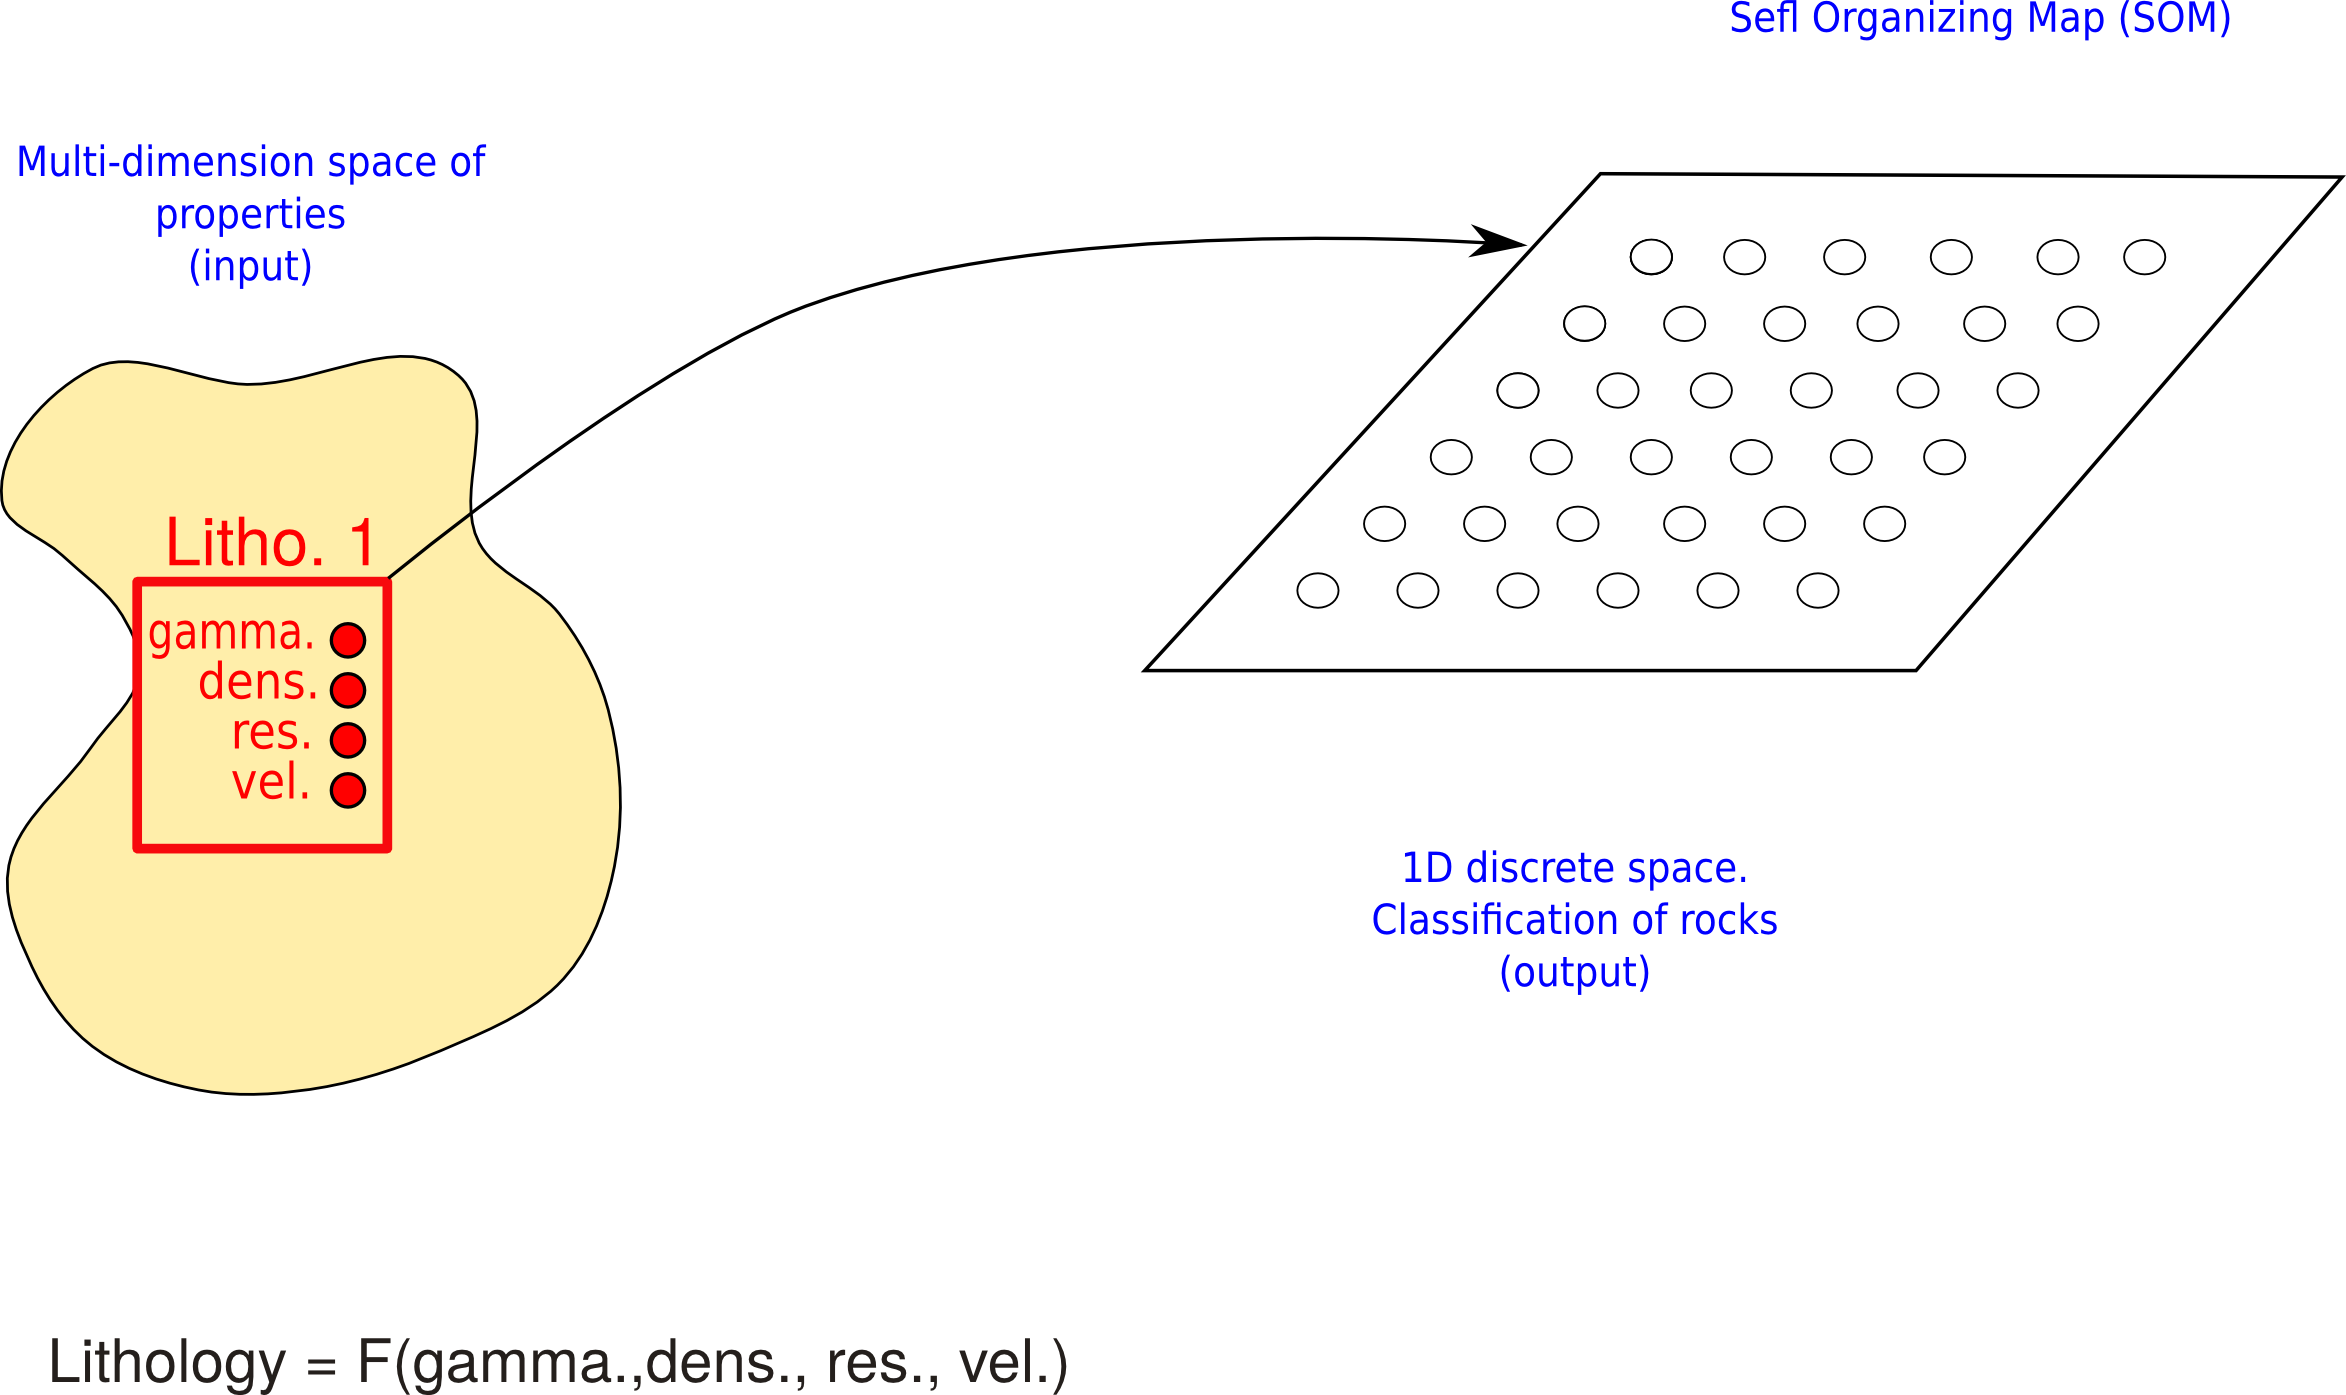
\includegraphics[scale=0.5]{Imagens/Introkoho3.png} 
\end{frame}


\begin{frame}
	\frametitle{Kohonen - SOM}
	\framesubtitle{Training}
	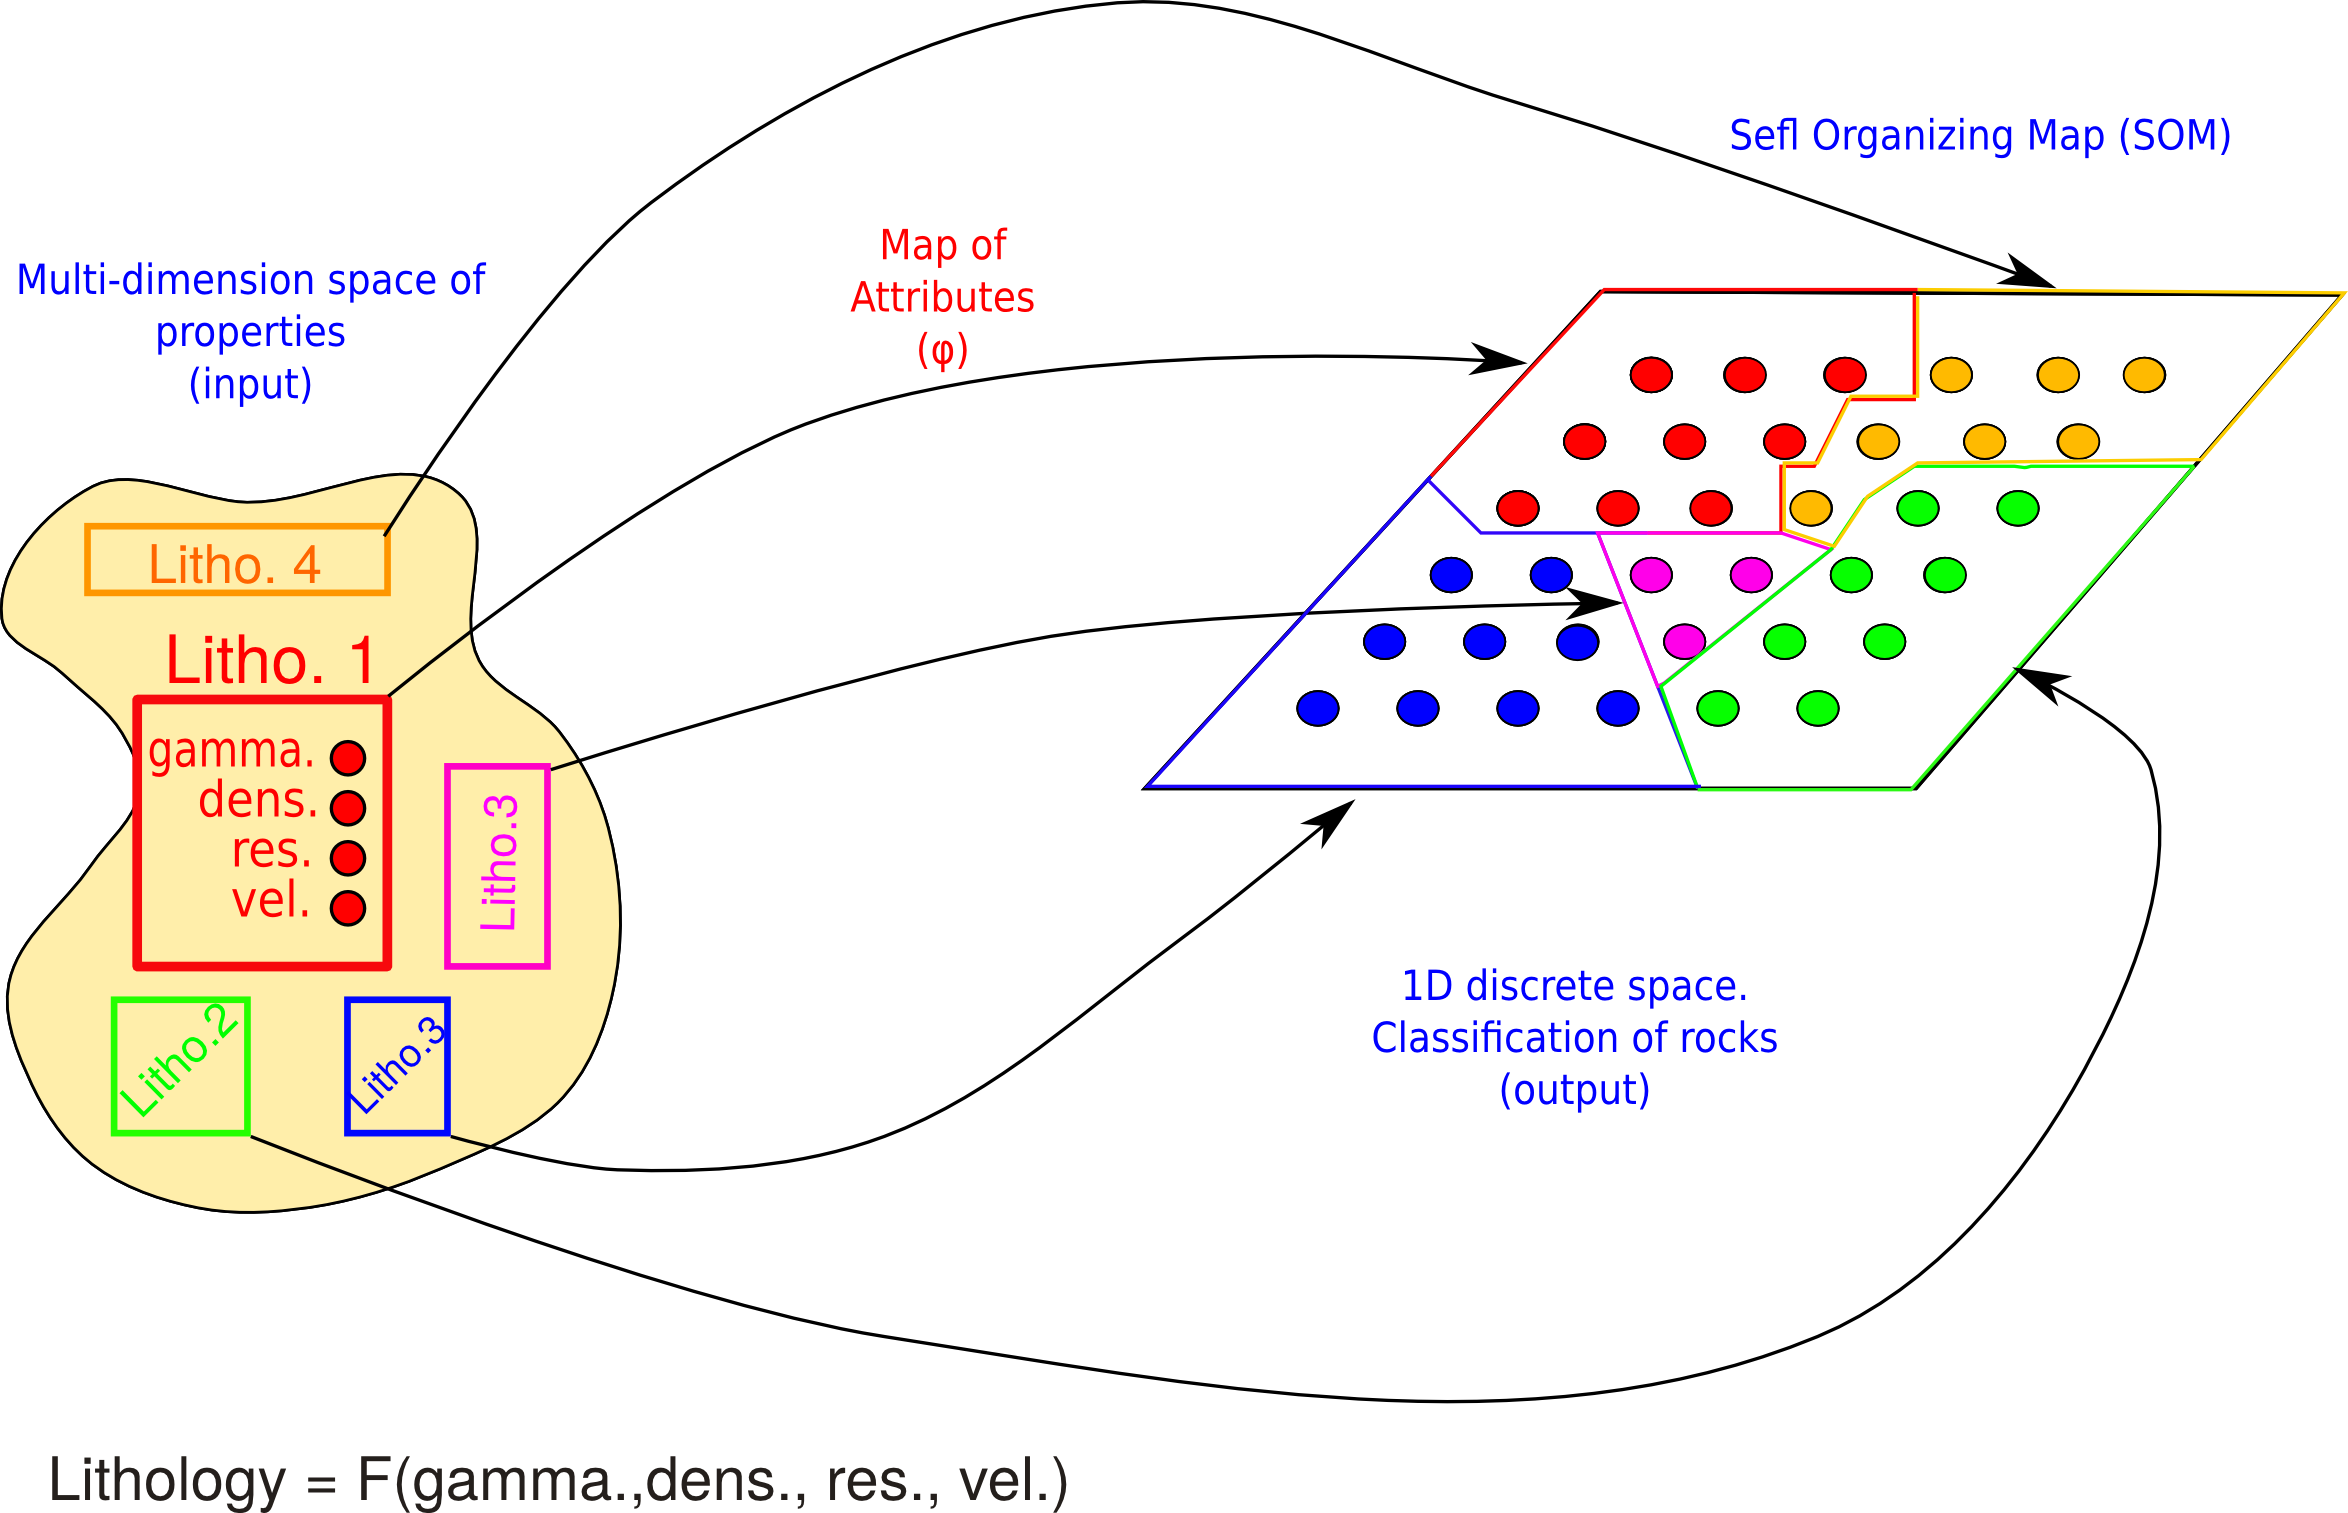
\includegraphics[scale=0.5]{Imagens/Introkoho4.png} 
\end{frame}

\begin{frame}
	\frametitle{Kohonen - SOM}
	\framesubtitle{Organization}

	\begin{eqnarray}
	\textbf{x}=[x_{1}, x_{2}, x_{3}, ..., x_{m}]^{T} \nonumber
	\end{eqnarray}
	\pause
	\begin{itemize}
		\centering
		\item[x], input data 
		\pause
	\end{itemize}
	\begin{eqnarray}
	\textbf{w}_{i,j}= [w_{j1}, w_{j2}, w_{j3}, ..., w_{jm}]^{T} \nonumber
	\end{eqnarray}
	\pause
	\begin{itemize}
		\centering
		\item[w], neuron atribute matrix 
	\end{itemize}
	\begin{eqnarray}
	j=1,2,3,\hdots,l \nonumber
	\end{eqnarray}
\end{frame}

%\begin{frame}
%    \frametitle{Kohonen - SOM}
%    \framesubtitle{Cooperation and winner neuron}
%	\begin{eqnarray}
%	i(\textbf{x})= argmin_{j}  \parallel \textbf{x} - \textbf{w}_{i,j} \parallel_{2} \nonumber
%	\end{eqnarray}
%%	 or 
%%	\begin{eqnarray}
%%	d(t)= \sqrt{\sum^{n}_{i=1}[x(t)-w_{i,j}(t)]^{2}} \hspace{1cm}  (j = {1,..,m}), \nonumber
%%	\label{eq1}
%%	\end{eqnarray}
%	
%	\begin{itemize}
%		\centering
%		\item[i(x)], distance or identity of a neuron i
%	\end{itemize}
%
%\end{frame}



\begin{frame}
 \frametitle{Kohonen - SOM}
 \framesubtitle{Synaptic adaption or Training process}
%Neuron changes the value of the surrounding neurons inside a quartet geometry
%

\begin{tcolorbox}[colback=gray!5,colframe=blue!40!black,title=Definition]
\begin{equation}
w_{i,j}(t+1)=w_{i,j}(t)+\eta(t)[x(t)-w_{i,j}(t)] \nonumber
\label{eq2}
\end{equation}  
\end{tcolorbox}

\pause

\begin{itemize}
	\centering
	\item[$w_{i,j}(t+1)$],  updated neuron attribute matrix
	\item[$\eta(t)$], learning rate
\end{itemize}
\pause
\begin{tcolorbox}[colback=gray!5,colframe=blue!40!black,title=Definition]
\begin{equation}
\eta(t)=\eta(0)    ( 1 -  \frac{t}{T}  ) \nonumber
\label{eq3}
\end{equation}  
\end{tcolorbox}

\begin{itemize}
	\centering
	\item[$T$], number of training cyles
%	\pause
	\item[$t$], number of iteractions
	%\pause
	%\item A iteractive process $t=t+1$ goes on until $t \approx  T$. Once the process ends for one neuron it repeats it self for the surrounding neighbors \citep{YANG2009,Yan2014}.
\end{itemize}

%Where $T$ is the number of training cyles and $t$ is the number of iteractions. A iteractive process $t=t+1$ goes on until $t \approx  T$. Once the process ends for one neuron it repeats it self for the surrounding neighbors.

\end{frame}


\begin{frame}
\frametitle{The geometry}

\begin{columns}
\column{0.2\textwidth}
\begin{figure}[H]
\flushleft
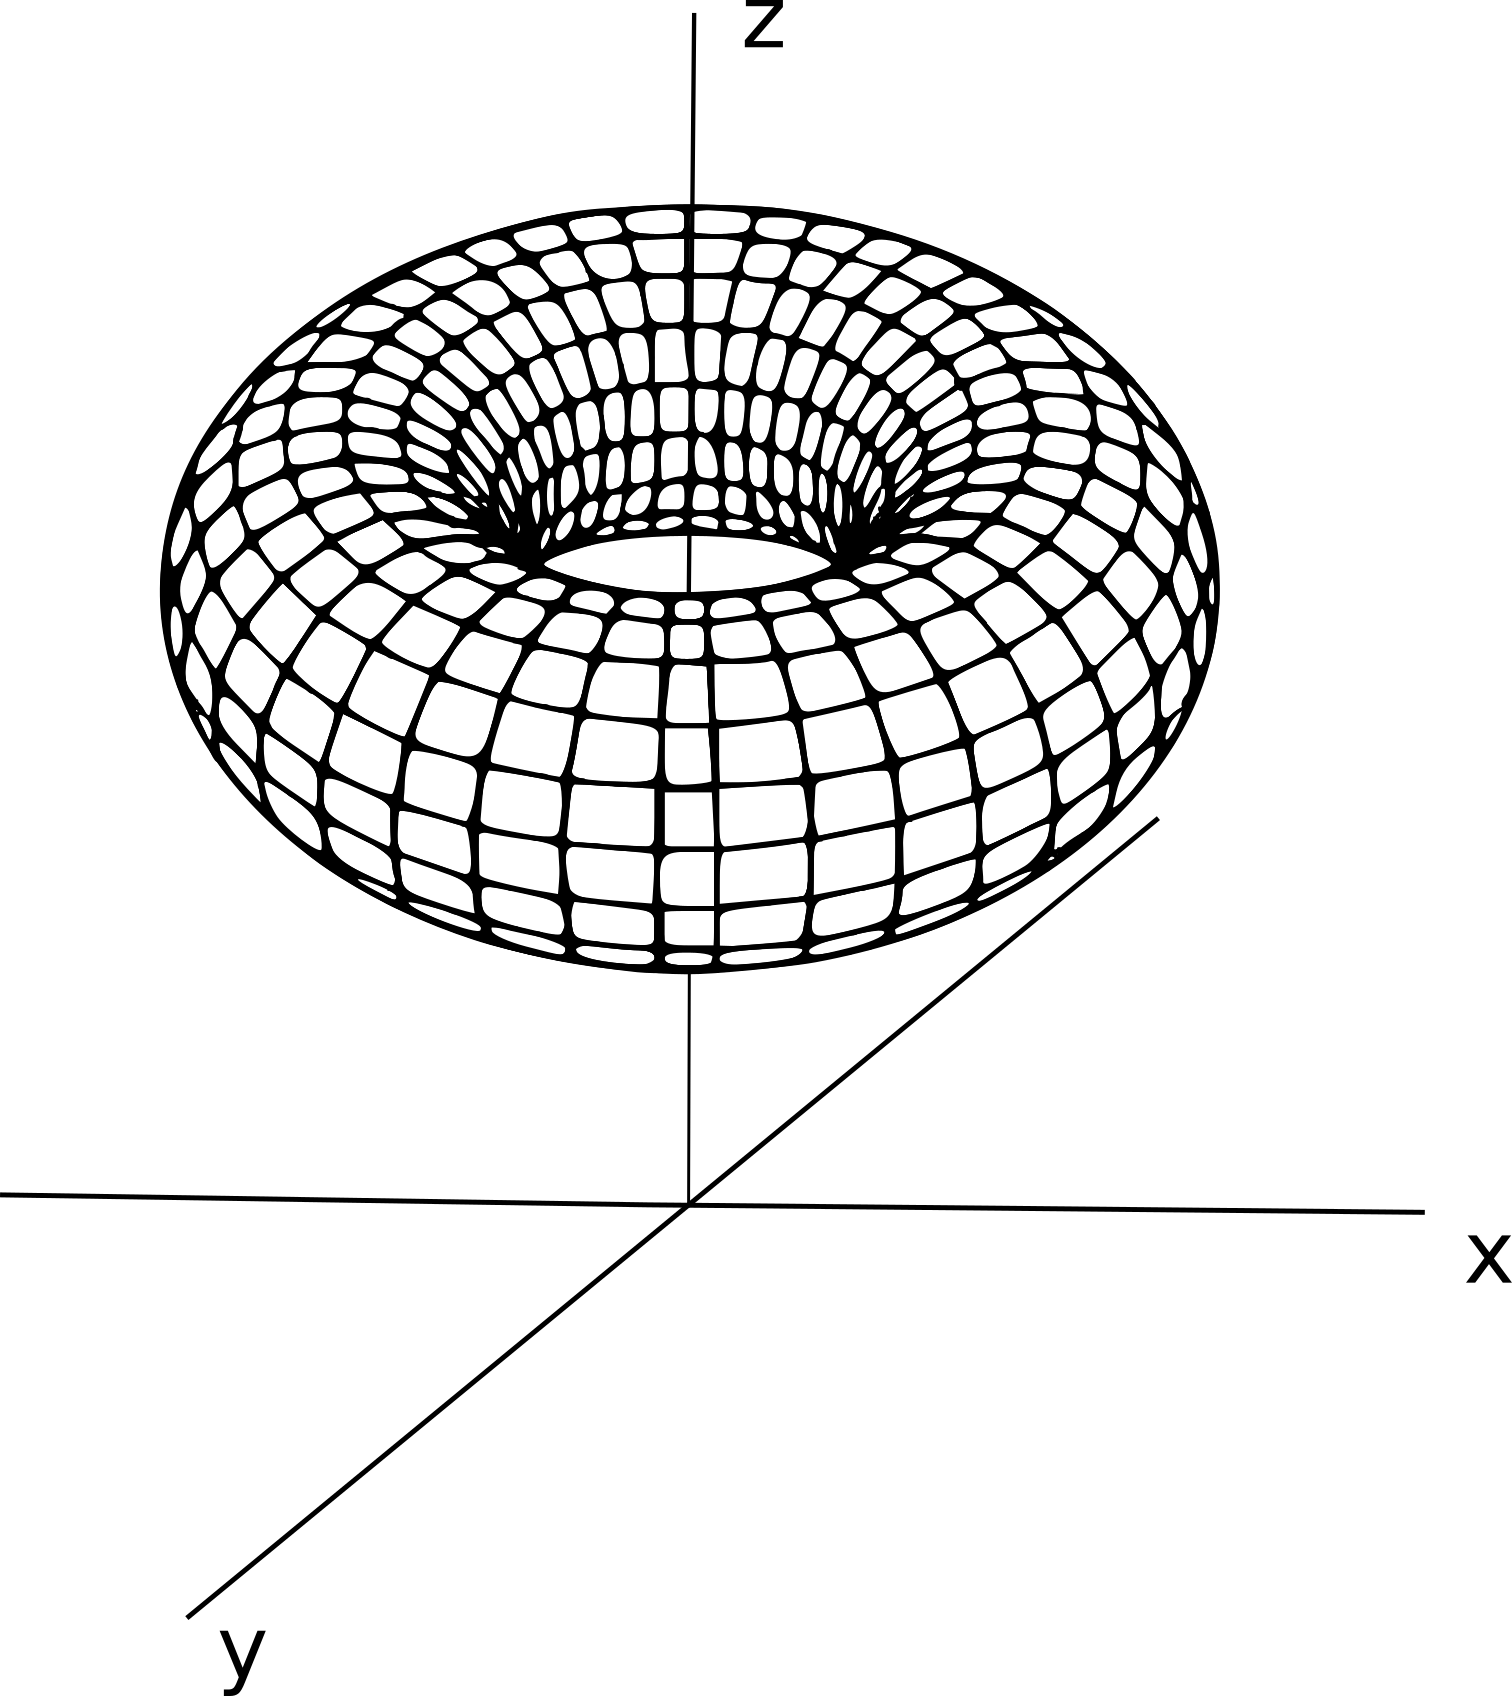
\includegraphics[scale=0.2]{Imagens/toro.png}
\label{toro}
\end{figure}
\column{0.5\textwidth}
\begin{figure}
\flushright
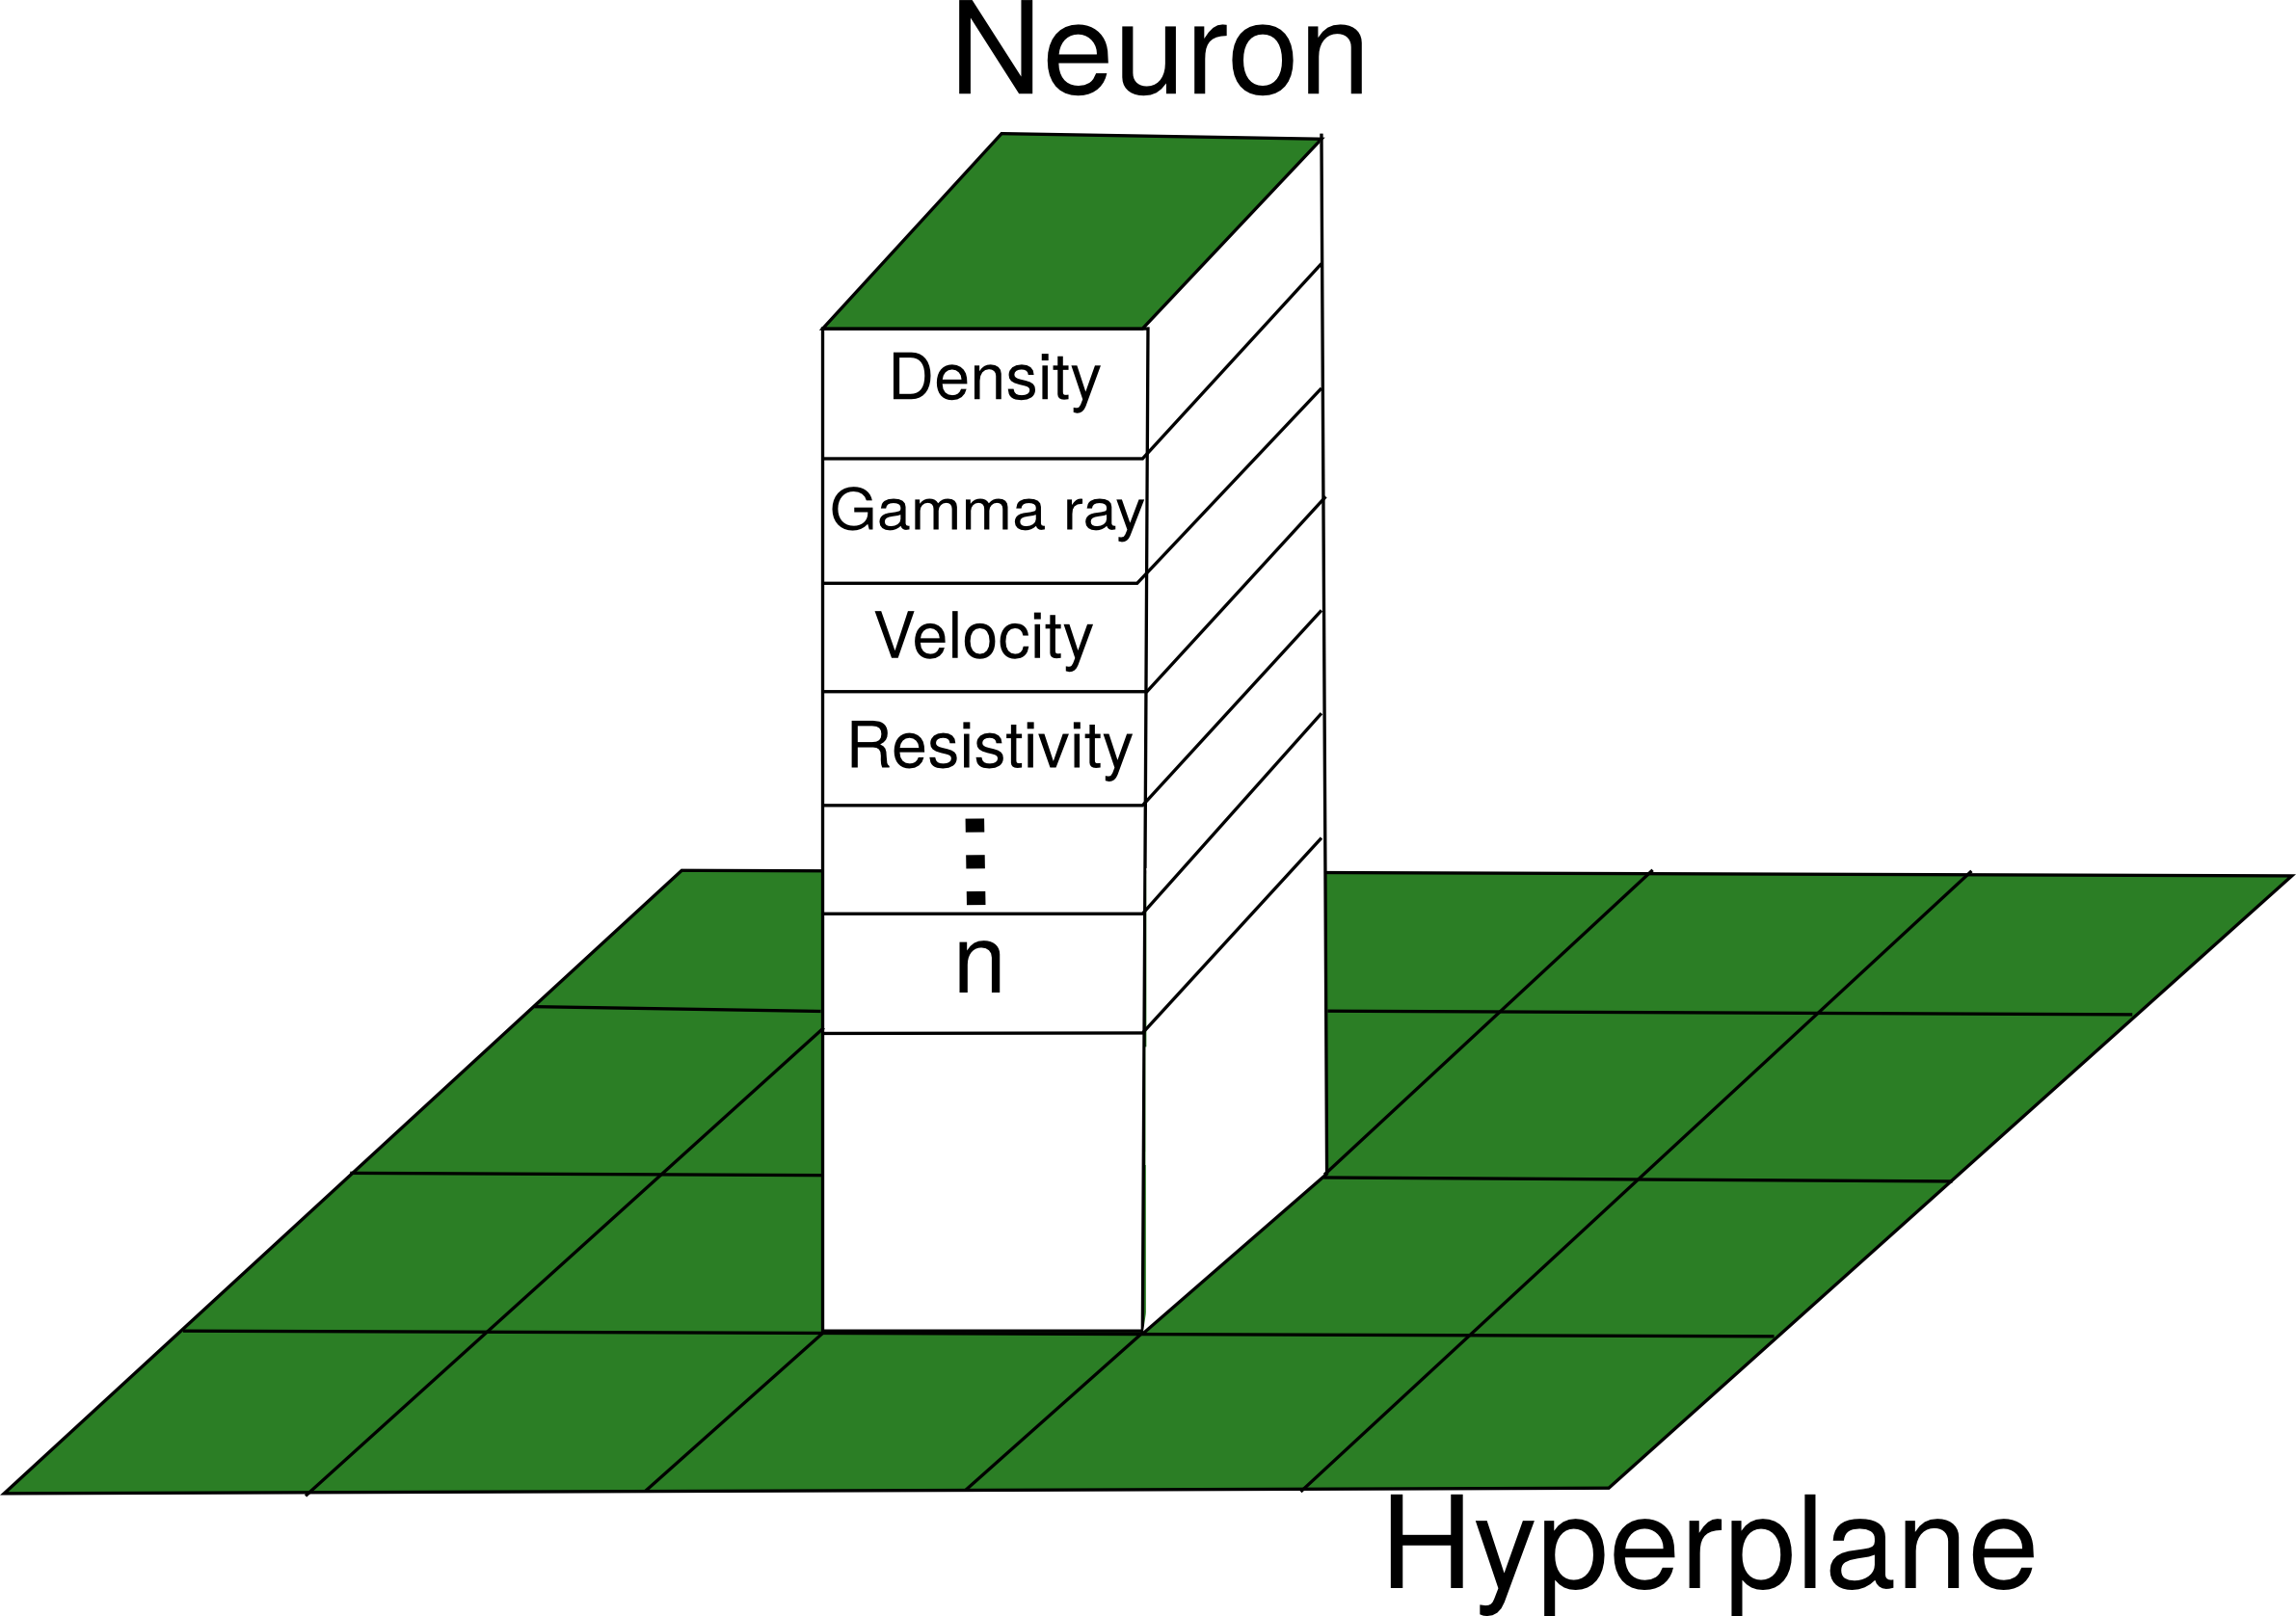
\includegraphics[scale=0.3]{Imagens/hiperplano.png}
\label{hiperplano}
\end{figure}
\end{columns}
\pause
\begin{itemize}
	\footnotesize
	\centering
	\item[Toroid], efficient way to connect all cells
	\item[Hyperplane], all attribute data goes here
\end{itemize}
\end{frame}


\begin{frame}
	\frametitle{Winner neuron and neighborhood}	
	\begin{eqnarray}
	i(\textbf{x})= argmin_{j}  \parallel \textbf{x} - \textbf{w}_{i,j} \parallel_{2} \nonumber
	\end{eqnarray}
	\begin{figure}
		\centering
		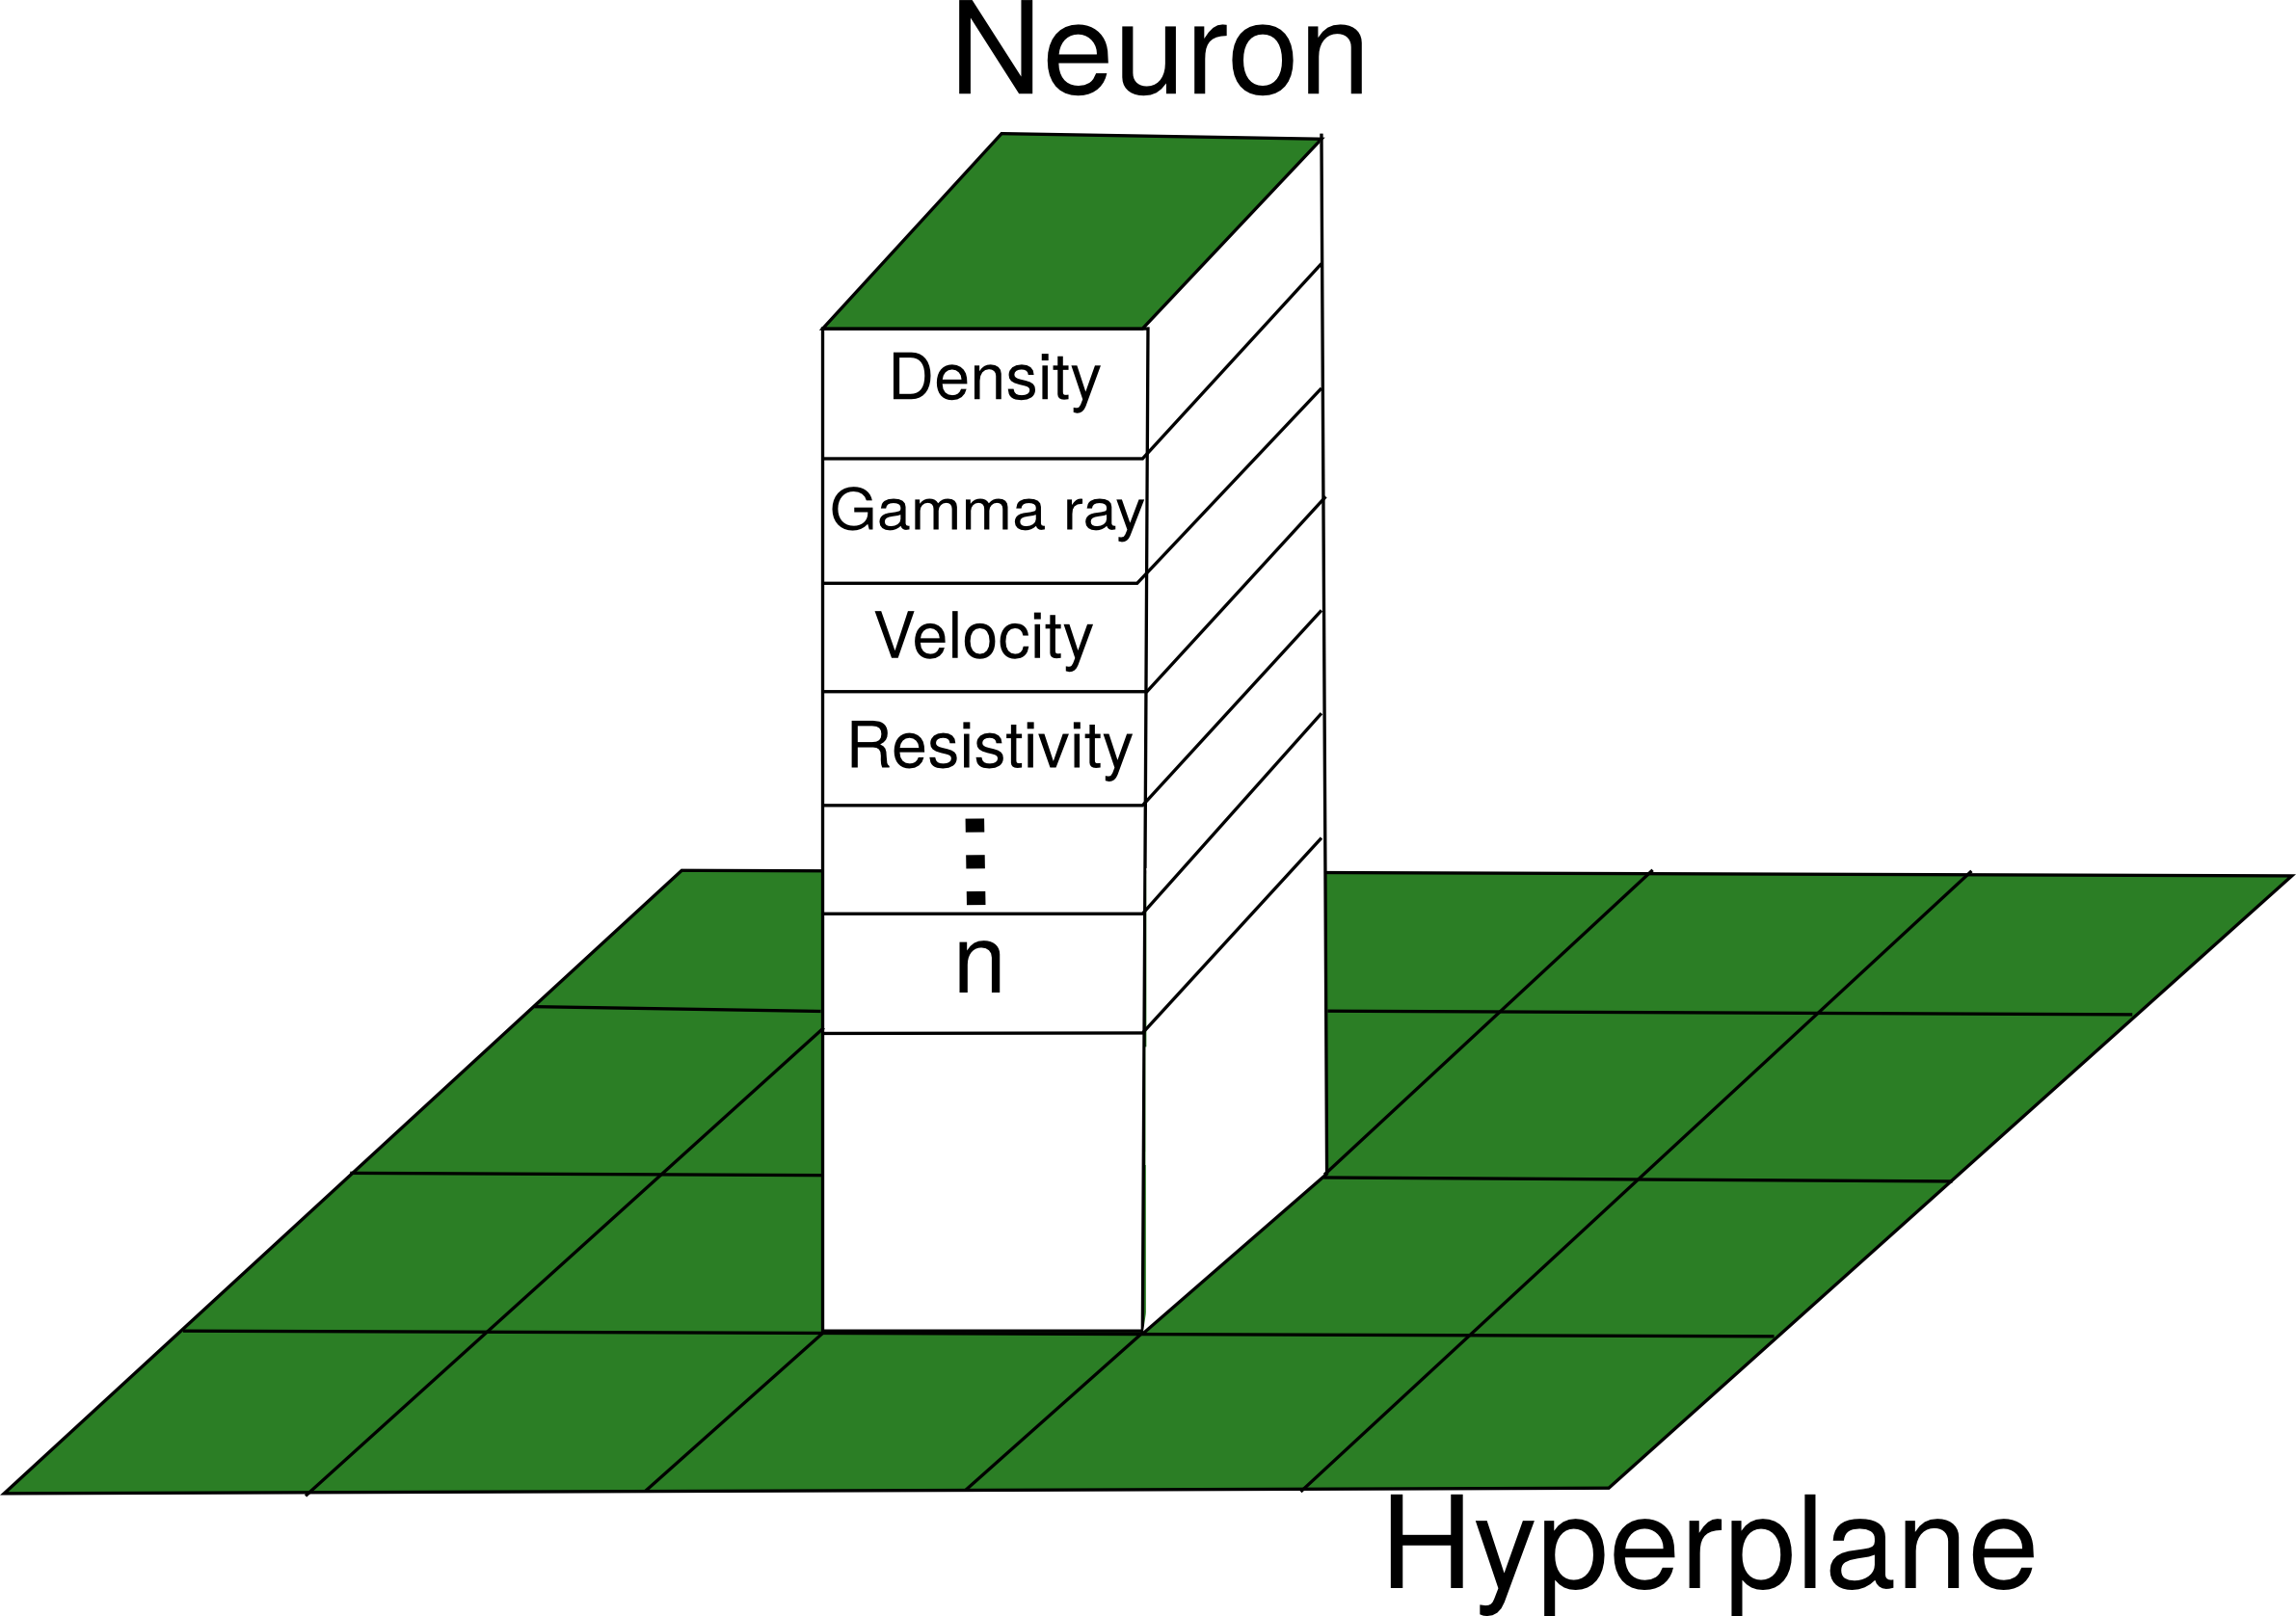
\includegraphics[scale=0.33]{Imagens/hiperplano.png}
		\label{vencedor1}
	\end{figure}
\end{frame}

\begin{frame}
	\frametitle{Winner neuron and neighborhood}
	\begin{eqnarray}
	i(\textbf{x})= argmin_{j}  \parallel \textbf{x} - \textbf{w}_{i,j} \parallel_{2} \nonumber
	\end{eqnarray}
	\begin{figure}
		\centering
		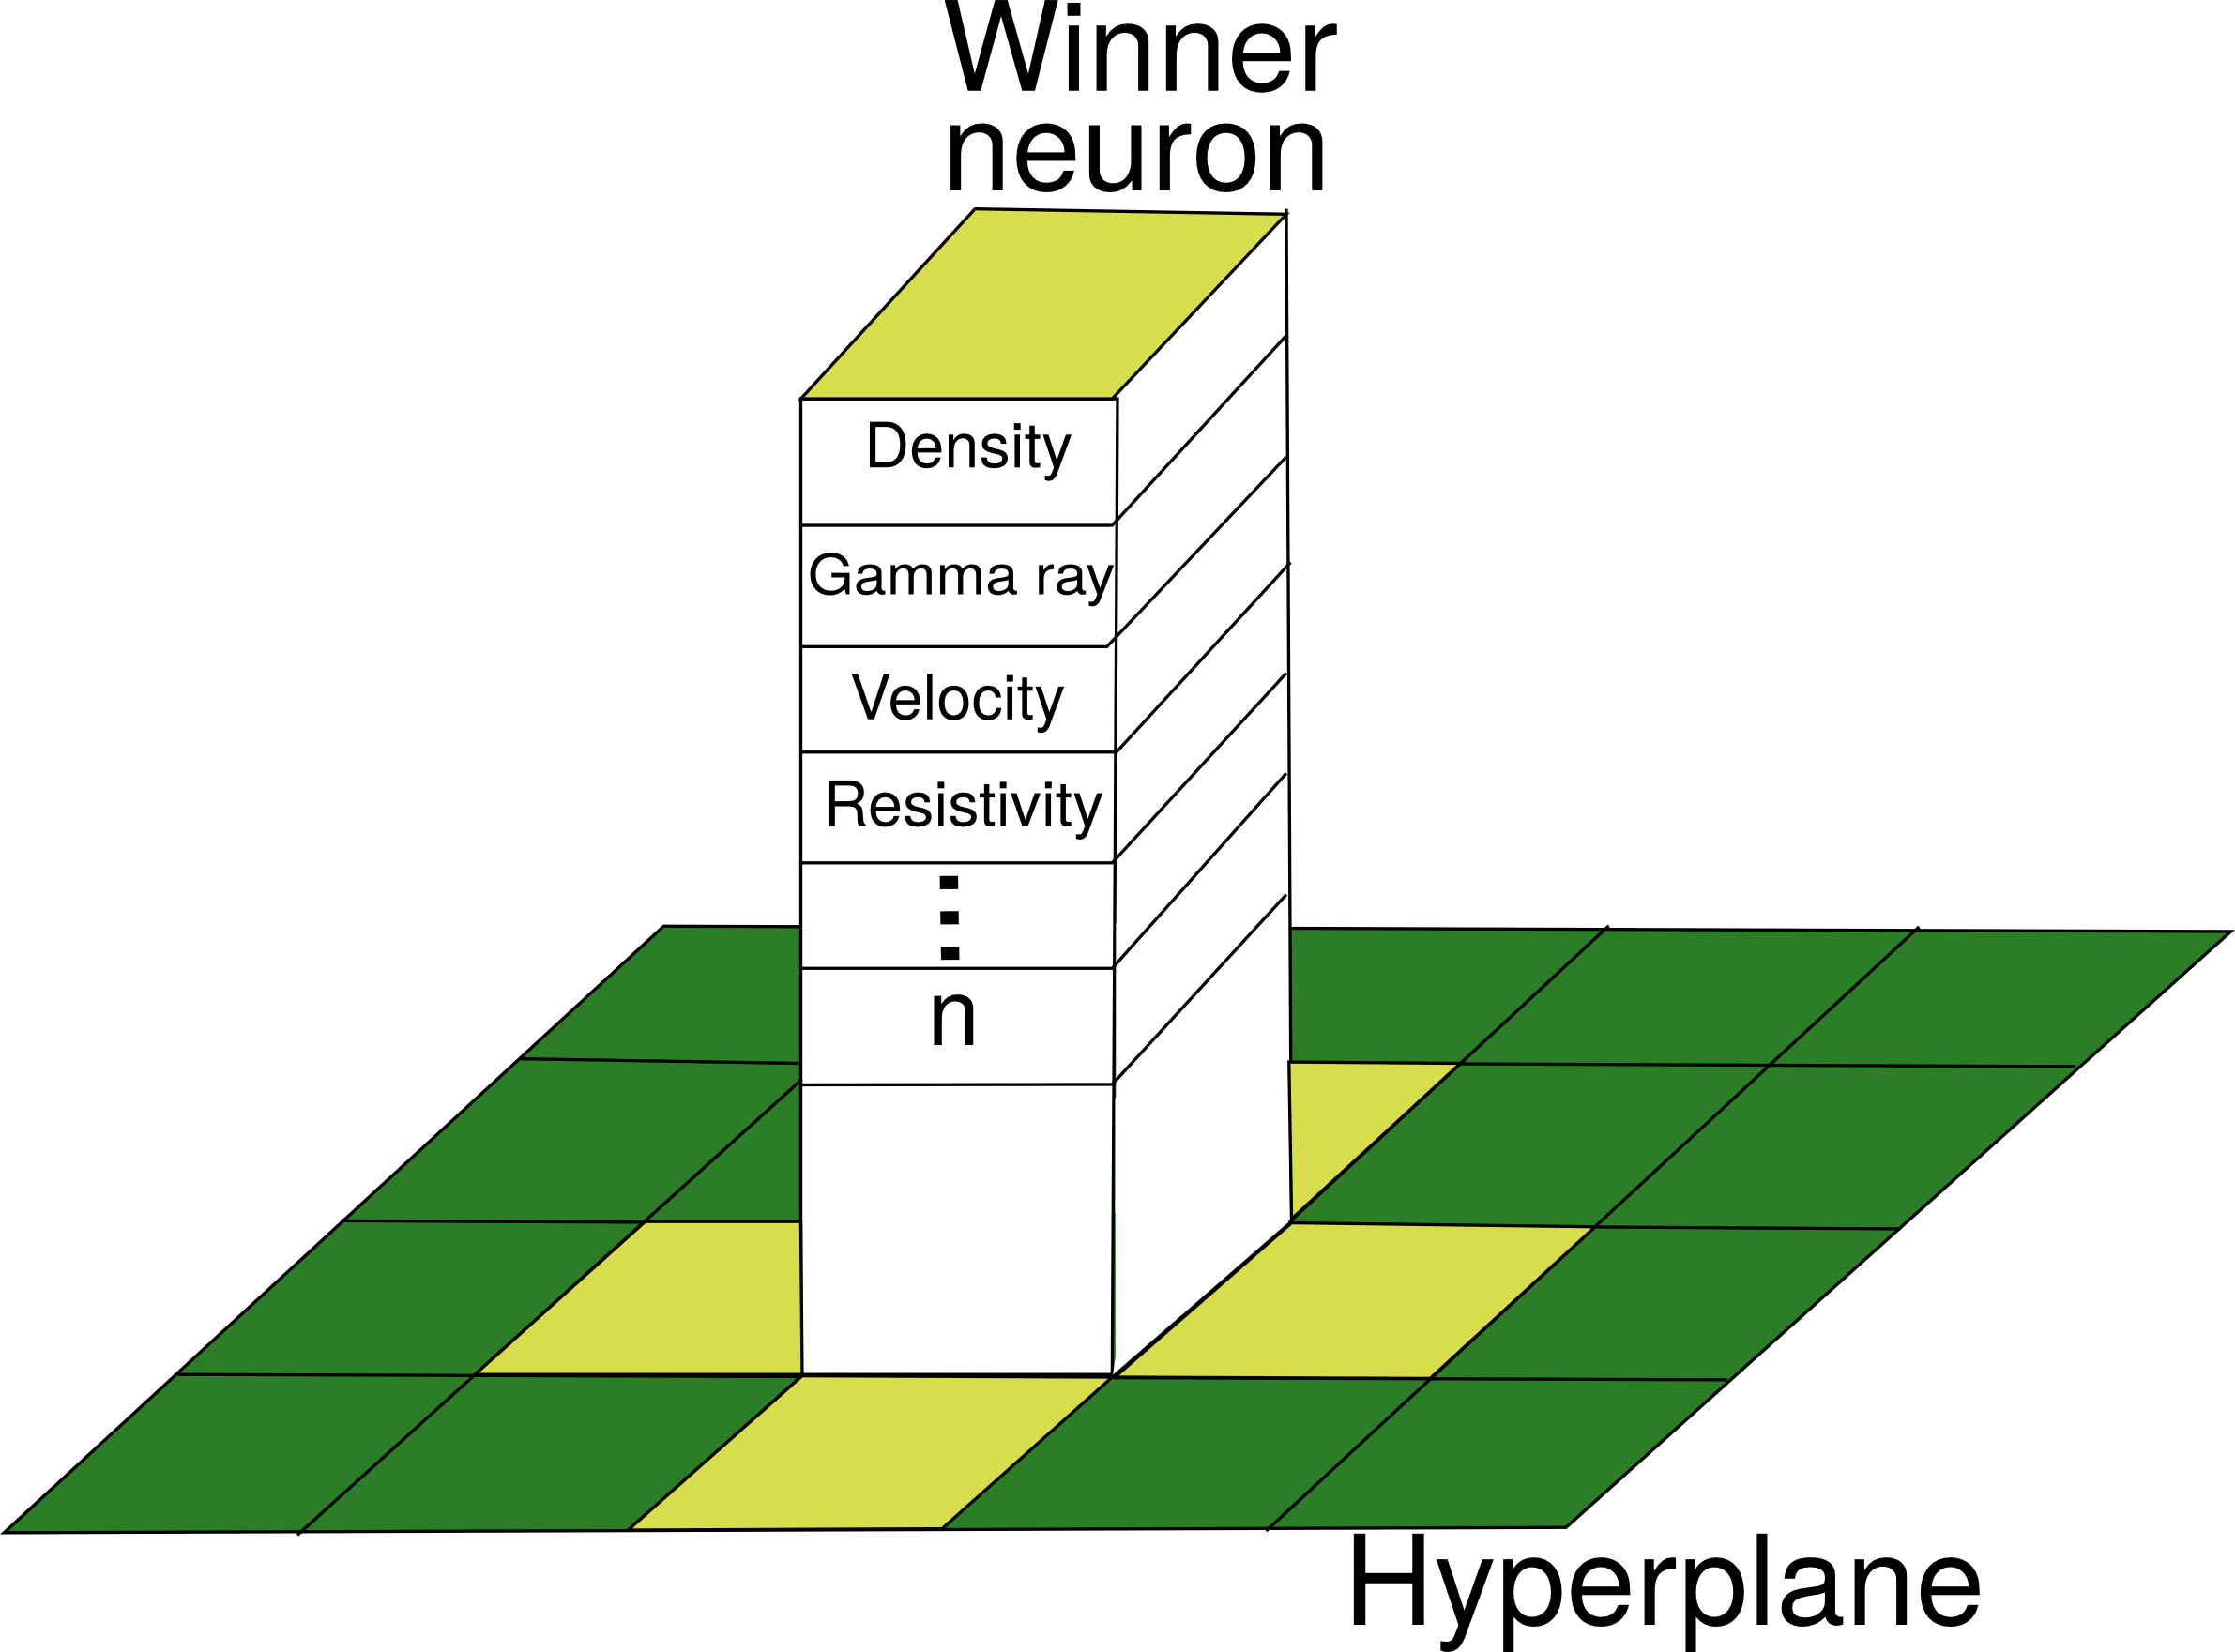
\includegraphics[scale=0.33]{Imagens/winner.png}
		\label{vencedor2}
	\end{figure}
\end{frame}

%\begin{frame}
%	\frametitle{A hyperplane with $400$ neurons}
%	\begin{table}[H]
%		\centering
%		\begin{tabular}{c|c}
%			
%			Lithology                   & Normalization \\ % Note a separação de col. e a quebra de linhas
%			\hline                                                             % para uma linha horizontal
%			Shale 2              &  1 \\
%			Dolomite  		     &  2 \\
%			Diabase    	         &  3 \\
%			Conglomerate         &  4 \\
%			Conglomerate 80\%    &  5 \\
%			Conglomerate 60\%    &  6 \\
%			Conglomerate 40\%    &  7 \\
%			Conglomerate 20\%    &  8 \\
%			Crystalline Basement &  9 \\
%			% não é preciso quebrar a última linha
%			
%		\end{tabular}
%		\label{codigos}
%		%\caption{Tabela de referência para conversão do padrão numérico em litologia.}
%	\end{table}
%\end{frame}

\begin{frame}
\frametitle{Training process for the synthetic case}
\framesubtitle{Epoch $5$}
\centering
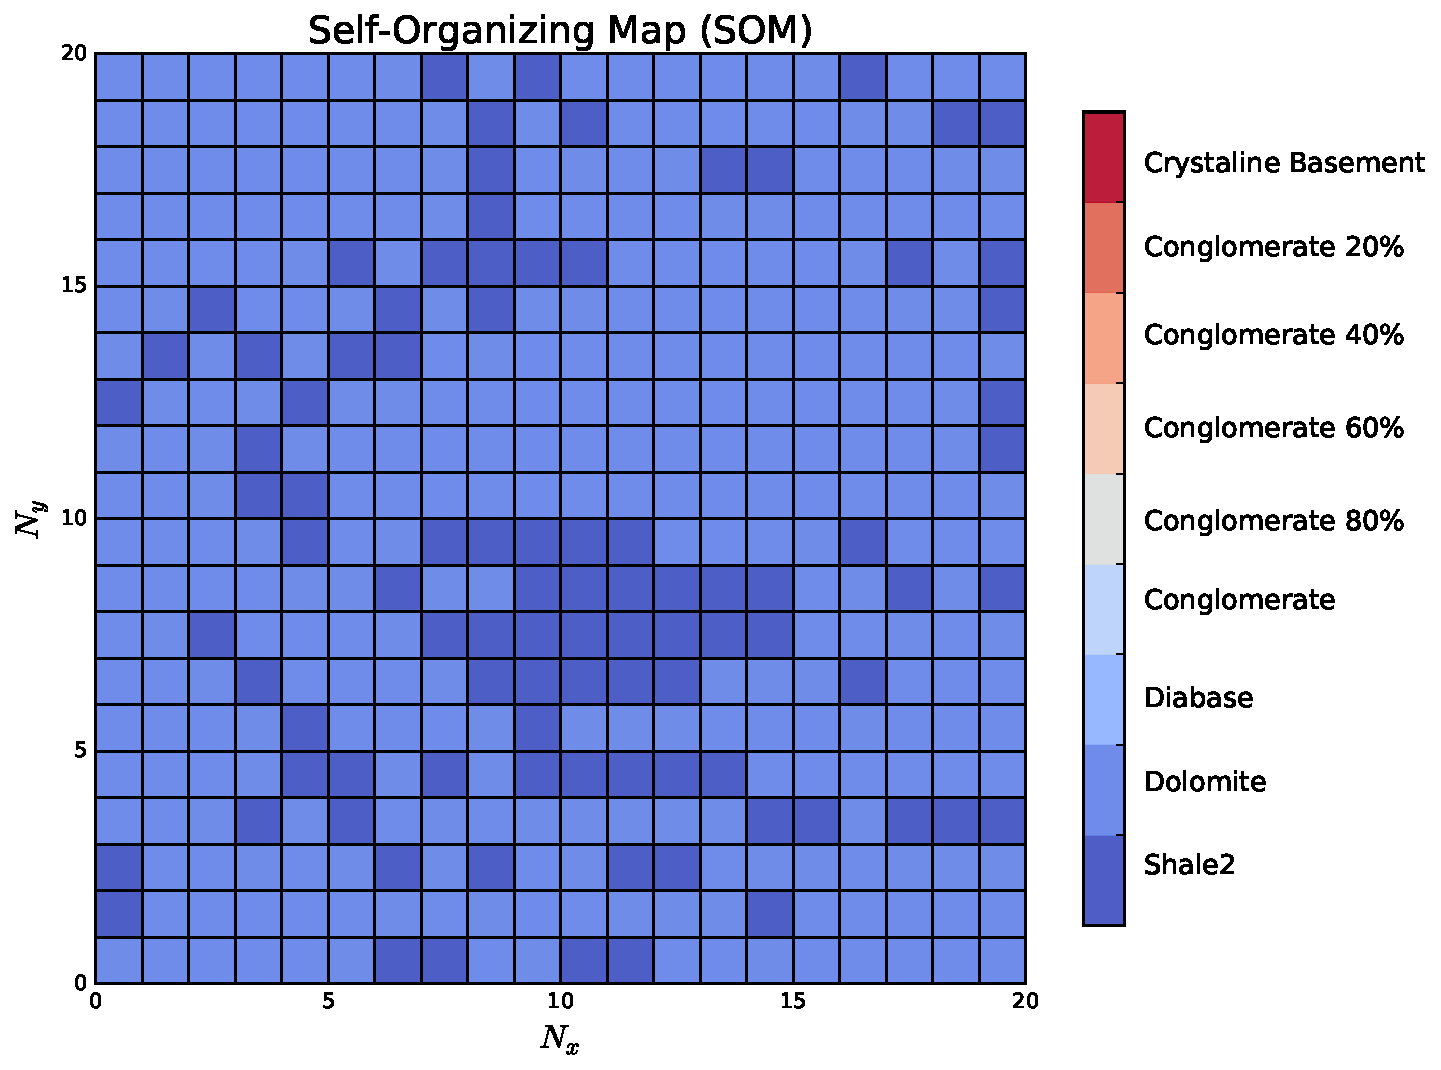
\includegraphics[scale=0.3]{Imagens/SOM5.pdf} 
\pause
\begin{itemize}
	\footnotesize
	%\centering
	\item $400$ neurons comprising the hyperplane
	\pause
	\item Epoch = iteraction in the training process
\end{itemize}
\end{frame}

\begin{frame}
\frametitle{Training process for the synthetic case}
\framesubtitle{Epoch $500$}
\centering
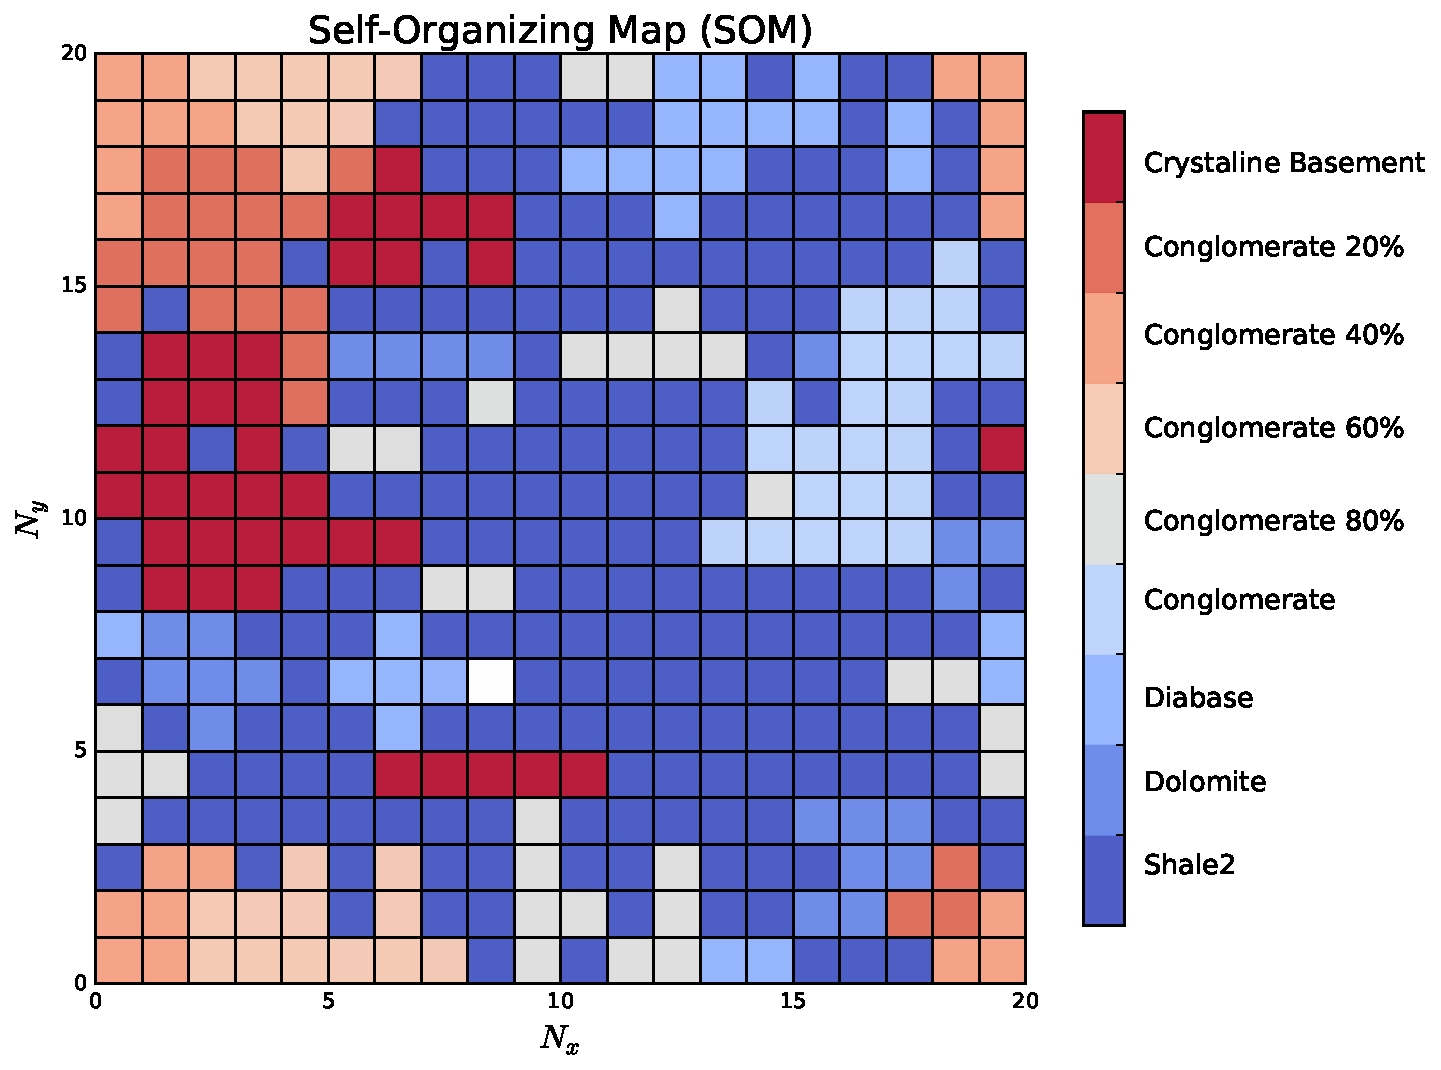
\includegraphics[scale=0.3]{Imagens/SOM100.pdf} 
\pause
\begin{itemize}
	\footnotesize
	%\centering
	\item Shale is the predominant rock in this stage
\end{itemize}
\end{frame}

\begin{frame}
\frametitle{Training process for the synthetic case}
\framesubtitle{Epoch $1000$}
\centering
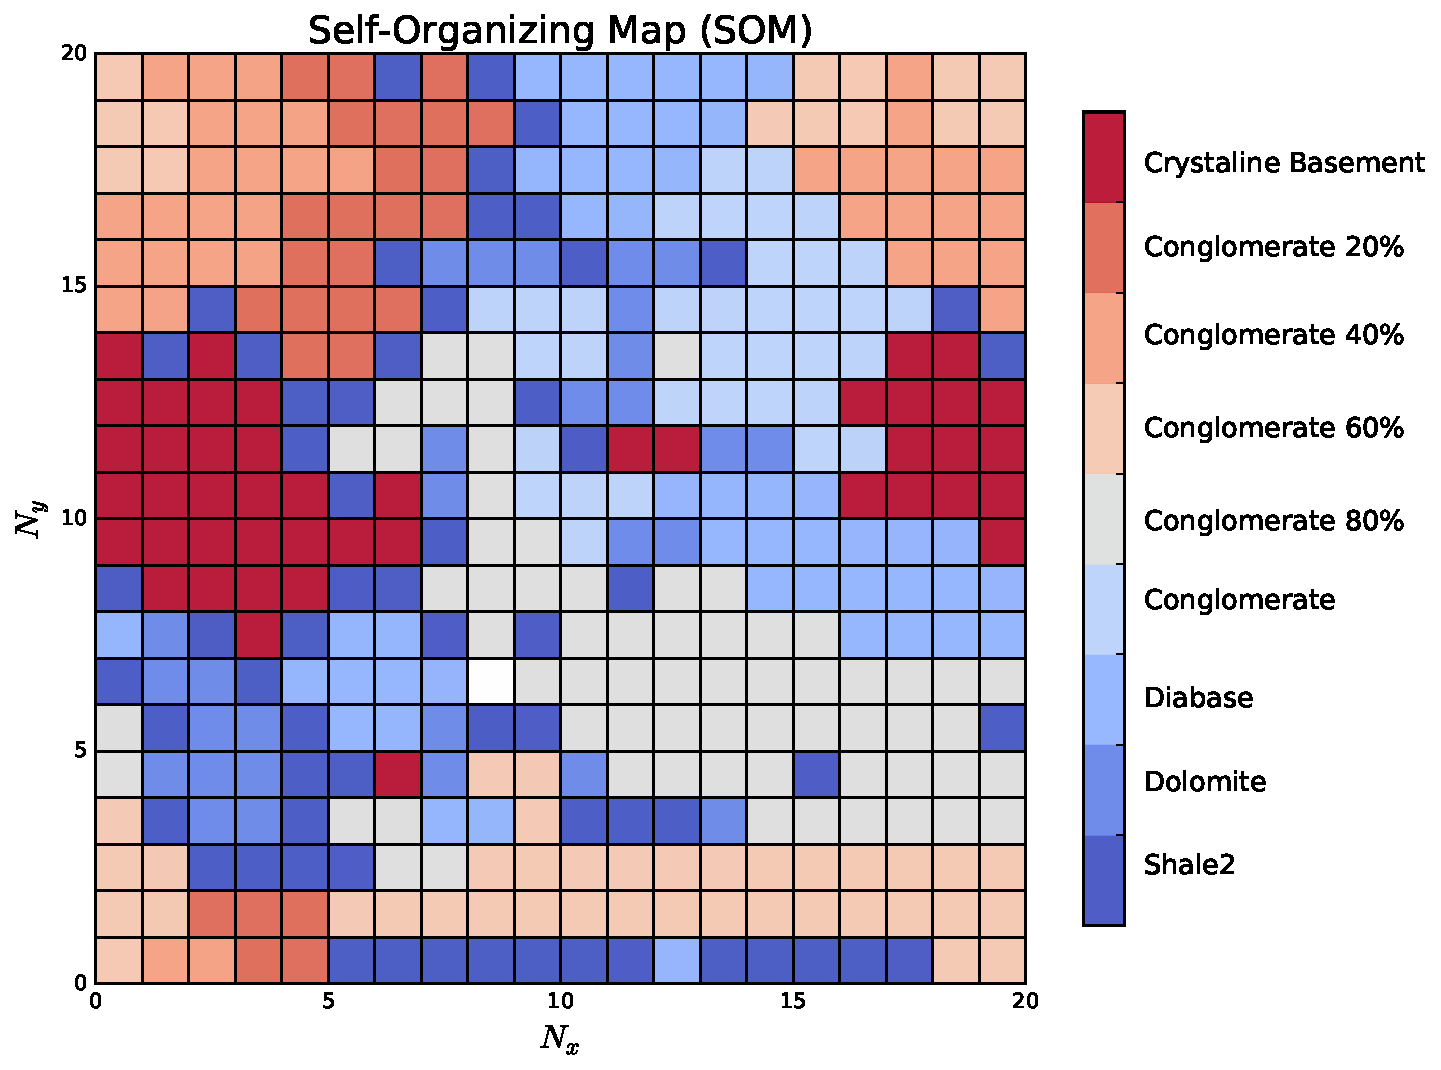
\includegraphics[scale=0.3]{Imagens/SOM1000.pdf} 
\pause
\begin{itemize}
	\footnotesize
	%\centering
	\item Final stage.
\end{itemize}
\end{frame}

%\begin{frame}
%\frametitle{Training process for the synthetic case}
%\framesubtitle{Convergence}
%%\centering
%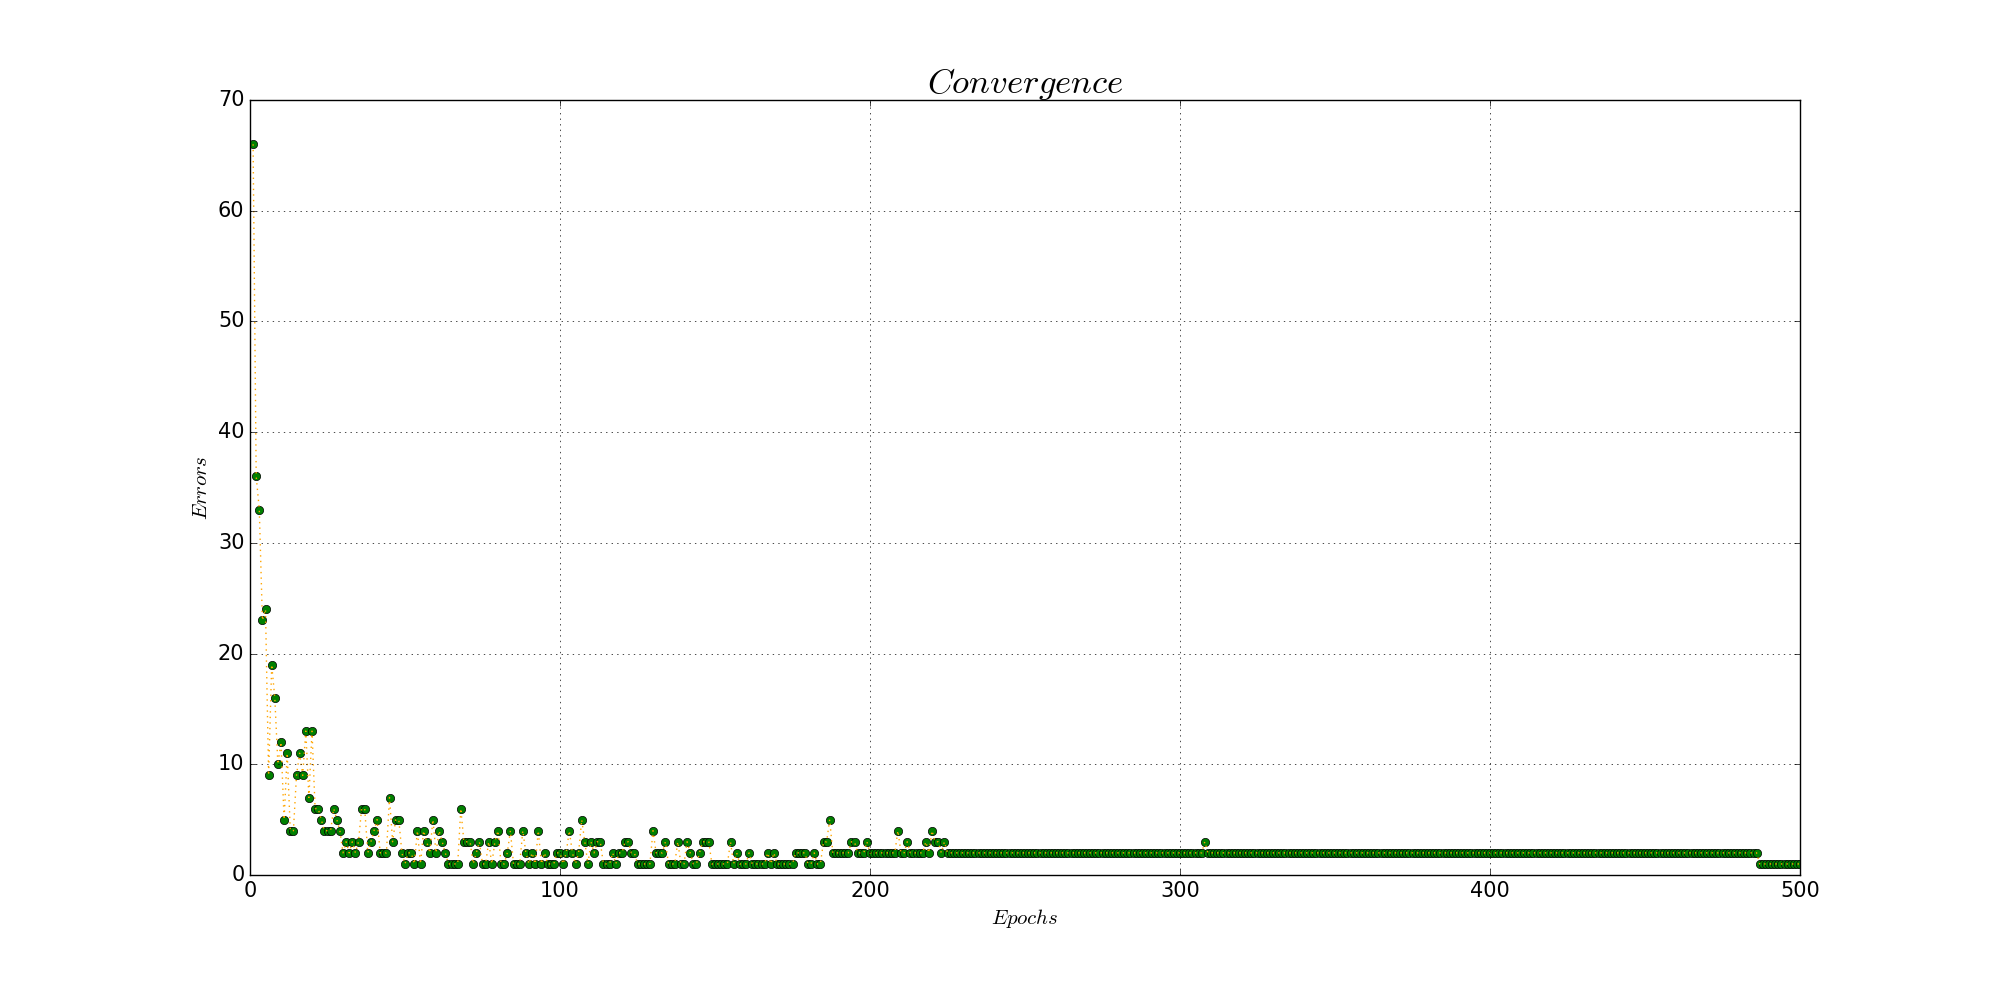
\includegraphics[scale=0.2]{Imagens/convEAGE18.png} 
%\end{frame}




\section{Results}

\begin{frame}
\frametitle{Results}
\framesubtitle{Classifications C1}
	\begin{figure}[H]
		\centering
		 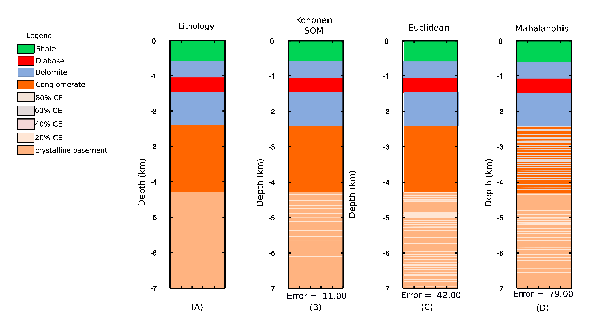
\includegraphics[scale=0.35]{Imagens/IDC1020118.eps}
		\caption{$700$ data measured in each well}
		\label{C1}
	\end{figure}
	\pause
\begin{eqnarray}
	Error=Lithology(z)-classification(z) \nonumber
\end{eqnarray}
\end{frame}

\begin{frame}
\frametitle{Results}
\framesubtitle{Classifications C2}
	\begin{figure}[H]
		\centering
		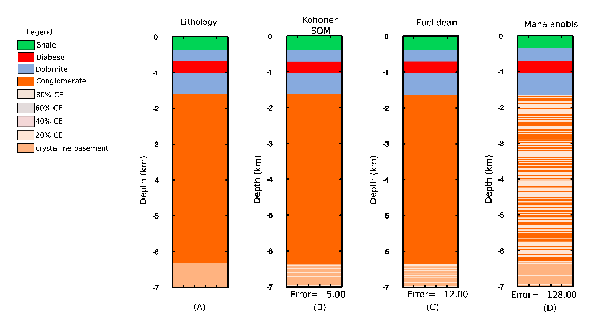
\includegraphics[scale=0.35]{Imagens/IDC2020118.eps}
        \caption{$700$ data measured in each well}
		\label{C2}
	\end{figure}
		\pause
		\begin{eqnarray}
		Error=Lithology(z)-classification(z) \nonumber
		\end{eqnarray}
\end{frame}

\begin{frame}
	\frametitle{Results}
	\framesubtitle{Comparative table}
		\begin{table}[H]
			\centering
			\begin{tabular}{||c|c|c|c||}
				\hline
Well &  SOM($\%$) & Euclidean($\%$) & Mahalanobis($\%$)\\ [0.5ex] \hline\hline 
C$1$	  &  1.57      &     6           &    11.28   \\
\hline
C$2$     &  0.71      &    1.71         &    18.28    \\ [1ex] 
\hline
				% não é preciso quebrar a última linha
			\end{tabular}
			\label{codigos}
			%\caption{Tabela de referência para conversão do padrão numérico em litologia.}
            \end{table}
\end{frame}

\section{Conclusions}

\begin{frame}
	\frametitle{Conclusions}
	\begin{itemize}
	%	\item SOM algorithm overperformed the euclidean and mahalanobis classifiers with an error of $0.71\%$
	%	\pause
		\item The complex distribution of features in the space of properties led to errors of $18.28\%$ (mahalanobis) and $1.71\%$ (euclidean) in the best scenario (C$2$ well).
		\pause
		\item Classifiers could not perform classification of bell patterns in well data. 
		\pause
		\item Box patterns could be solved by euclidean classifier but not by mahalanobis
		\pause
		\item Kohonen SOM showed better performance concerning classification of mixture of rocks or the bell pattern
	\end{itemize}
\end{frame}

\section{Future Perspectives}

\begin{frame}
	\frametitle{Future Perspectives}
	\begin{itemize}
		\pause
		\item Make more tests with more training wells to verify why such a poor performance of Mahalanobis Classifier;
		\pause
		\item Create a more promising stop criterion for the training process (in development);
		\pause
		\item Real data application (Paraná Sedimentary Basin, Southeast Brazil)
	\end{itemize}
\end{frame}

%\section{References}

\begin{frame}[allowframebreaks]
\frametitle{References}
%\beamertemplatetextbibitems
\tiny
\bibliographystyle{apalike}
\bibliography{references}
\end{frame}

\begin{frame}
\flushbottom
\setlength{\parskip}{-1ex plus 1ex }
\setlength{\parindent}{-15pt}
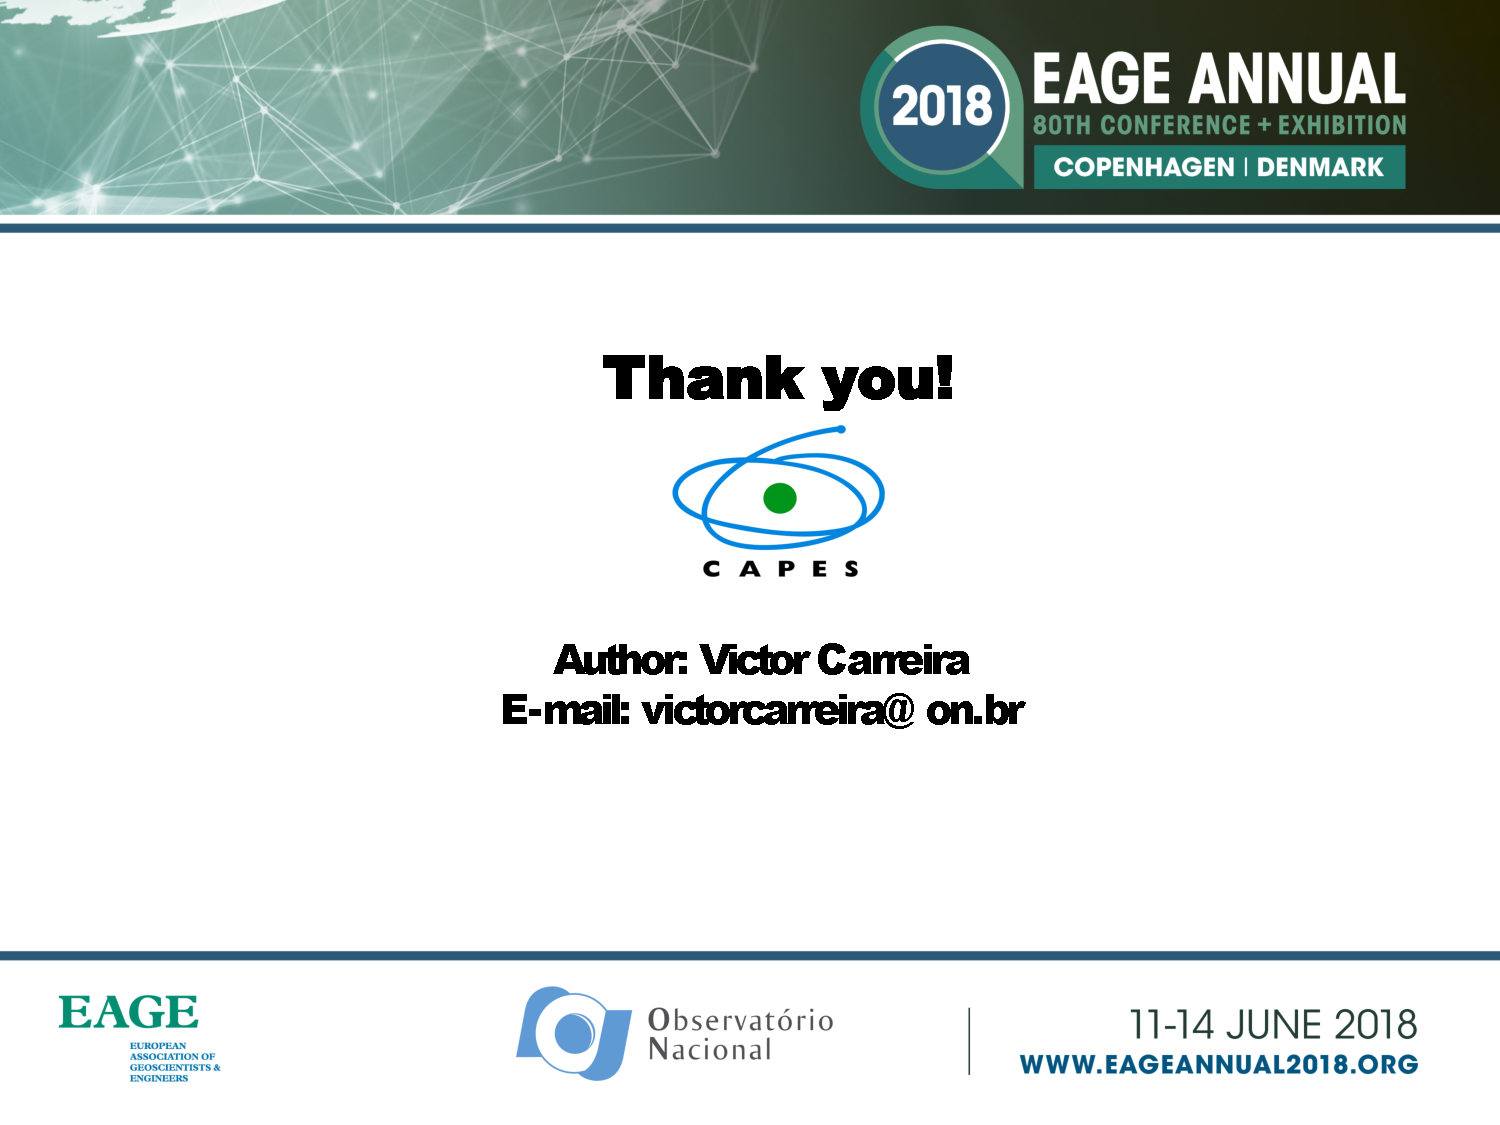
\includegraphics[width=13cm,height=10cm]{Imagens/end.pdf}
\end{frame}

\end{document}